\documentclass{article}

\usepackage{fancyhdr}
\usepackage{extramarks}
\usepackage{amsmath}
\usepackage{amsthm}
\usepackage{amsfonts}
\usepackage{tikz}
\usepackage{enumerate}
\usepackage{graphicx}
\graphicspath{ {images/} }
\usepackage[plain]{algorithm}
\usepackage{algpseudocode}
\usepackage[document]{ragged2e}
\usepackage{textcomp}
\usepackage{color}   %May be necessary if you want to color links
\usepackage{hyperref}
\hypersetup{
    colorlinks=true, %set true if you want colored links
    linktoc=all,     %set to all if you want both sections and subsections linked
    linkcolor=black,  %choose some color if you want links to stand out
}

\usetikzlibrary{automata,positioning}

%
% Basic Document Settings
%

\topmargin=-0.45in
\evensidemargin=0in
\oddsidemargin=0in
\textwidth=6.5in
\textheight=9.0in
\headsep=0.25in
\setlength{\parskip}{1em}

\linespread{1.1}

\pagestyle{fancy}
\lhead{\hmwkAuthorName}
%\chead (\hmwkTitle}
%\rhead{\firstxmark}
\lfoot{\lastxmark}
\cfoot{\thepage}

\renewcommand\headrulewidth{0.4pt}
\renewcommand\footrulewidth{0.4pt}

\setlength\parindent{0pt}

%
% Create Problem Sections
%

\newcommand{\enterProblemHeader}[1]{
    \nobreak\extramarks{}{Question \arabic{#1} continued on next page\ldots}\nobreak{}
    \nobreak\extramarks{Question \arabic{#1} (cont.)}{Question \arabic{#1} continued on next page\ldots}\nobreak{}
}

\newcommand{\exitProblemHeader}[1]{
    \nobreak\extramarks{Question \arabic{#1} (cont.)}{Question \arabic{#1} continued on next page\ldots}\nobreak{}
    \stepcounter{#1}
    \nobreak\extramarks{Question \arabic{#1}}{}\nobreak{}
}

\setcounter{secnumdepth}{0}
\newcounter{partCounter}
\newcounter{homeworkProblemCounter}
\setcounter{homeworkProblemCounter}{1}
\nobreak\extramarks{Problem \arabic{homeworkProblemCounter}}{}\nobreak{}

%
% Homework Problem Environment
%
% This environment takes an optional argument. When given, it will adjust the
% problem counter. This is useful for when the problems given for your
% assignment aren't sequential. See the last 3 problems of this template for an
% example.
%
\newenvironment{homeworkProblem}[1][-1]{
    \ifnum#1>0
        \setcounter{homeworkProblemCounter}{#1}
    \fi
    \section{Problem \arabic{homeworkProblemCounter}}
    \setcounter{partCounter}{1}
    \enterProblemHeader{homeworkProblemCounter}
}{
    \exitProblemHeader{homeworkProblemCounter}
}

%
% Homework Details
%   - Title
%   - Due date
%   - Class
%   - Section/Time
%   - Instructor
%   - Author
%

\newcommand{\hmwkTitle}{Math Review Notes}
%%\newcommand{\hmwkDueDate}{September 14, 2017}
%\newcommand{\hmwkClass}{Math 4650}
%\newcommand{\hmwkClassTime}{Section A}
%\newcommand{\hmwkClassInstructor}{A. Shaheen}
\newcommand{\hmwkAuthorName}{\textbf{G. Faletto} }

%
% Title Page
%

\title{
    \vspace{2in}
    \textmd{\textbf{ \hmwkTitle}}\\
%    \normalsize\vspace{0.1in}\small{Due\ on\ \hmwkDueDate}\\
%    \vspace{0.1in}\large{\textit{Instructor: Tony Shaheen\ }}
%    \vspace{3in}
}

\author{Gregory Faletto}
\date{}

\renewcommand{\part}[1]{\textbf{\large Part \Alph{partCounter}}\stepcounter{partCounter}\\}

%
% Various Helper Commands
%

% Useful for algorithms
\newcommand{\alg}[1]{\textsc{\bfseries \footnotesize #1}}

% For derivatives
\newcommand{\deriv}[2]{\frac{\mathrm{d} #1}{\mathrm{d} #2}}

% For partial derivatives
\newcommand{\pderiv}[2]{\frac{\partial #1}{\partial #2}}

% Integral dx
\newcommand{\dx}{\mathrm{d}x}

% Alias for the Solution section header
\newcommand{\solution}{\textbf{\large Solution}}

% Probability commands: Expectation, Variance, Covariance, Bias
\newcommand{\E}{\mathbb{E}}
\newcommand{\Var}{\mathrm{Var}}
\newcommand{\Cov}{\mathrm{Cov}}
\newcommand{\Bias}{\mathrm{Bias}}

% Tilde
\newcommand{\textapprox}{\raisebox{0.5ex}{\texttildelow}}

\begin{document}

\maketitle

\pagebreak

\tableofcontents

\newpage

% Linear Algebra
\section{Linear Algebra}
\subsection{Properties of Projection Matrices}

\begin{enumerate}[i.]

\item Formula:

\[
P = A(A^TA)^{-1}A^T
\]

(Note that if \(A\) is an invertible (square) matrix, then \(P = A(A^TA)^{-1}A^T = AA^{-1}(A^T)^{-1}A^T = I\).)

\textbf{The projection matrix projects any vector \(b\) into the column space of \(A\).} In other words, \(p = Pb\) is the component of \(b\) in the column space, and the error \(e = b - Pb\) is the component in the orthogonal complement. (\(I - P\) is also a projection matrix. It projects \(b\) onto the orthogonal complement, and the projection is \(b - Pb = e\)).

(Note that if \(A\) is an invertible (square) matrix, then its column space is all of \(\mathbb{R}^n\), so \(b\) is already in the column space of \(A\).)

\item The projection matrix is \textbf{idempotent}: it equals its square--\(P^2 = P\).

\item The projection matrix is \textbf{symmetric}: it equals its transpose--\(P^T = P\).

\item Conversely, \textbf{any symmetric idempotent matrix represents a projection}. \(P\) is unique for a given subspace.

\item If \(A\) is an \(m \times n\) matrix with rank \(n\), then \(\text{rank} (P) = n\). The eigenvalues of \(P\) consist of \(n\) ones and \(m - n\) zeroes. \(P\) always contains \(n\) independent eigenvectors and is thus diagonalizable. 

\end{enumerate}

Suppose \(A\) is a square nonsingular matrix and \(\lambda\) is an eigenvalue of \(A\). Then \(\lambda^{-1}\) is an eigenvalue of the matrix \(A^{-1}\).

The trace of an idempotent matrix with rank \(r\) is \(r\).

\subsection{Eigenvalues, Eigenvectors, Diagonalization, Symmetric Matrices}

\textbf{Notes on Diagonalization}

Suppose the \(n \times n\) matrix \(A\) has \(n\) linearly independent eigenvectors. If these eigenvectors are the columns of a matrix \(S\), then \(S^{-1}AS\) is a diagonal matrix \(\Lambda\). The eigenvalues of \(A\) are on the diagonal of \(\Lambda\):

\[
S^{-1}AS = \Lambda = \begin{bmatrix}
   \lambda_1       & 0  & \cdots  & 0  \\
  0  & \lambda_2 & \cdots  & 0 \\
  \vdots  & \vdots  & \ddots & \vdots \\
   0  & 0 & \cdots & \lambda_n
\end{bmatrix}
\]

We call \(S\) the \textbf{eigenvector matrix} and \(\Lambda\) the \textbf{eigenvalue matrix}.

\begin{enumerate}[1.]

\item If the matrix \(A\) has no repeated eigenvalues, then its \(n\) eigenvectors are automatically independent. Therefore \textbf{any matrix with \(n\) distinct eigenvalues can be diagonalized}.

\item \textbf{The diagonalizing matrix \(S\) is not unique}. An eigenvector \(x\) can be multiplied by a constant and remains an eigenvector. We can multiply the columns of \(S\) by any nonzero constants and produce a new diagonalizing \(S\). Repeated eigenvalues leave even more freedom in \(S\) (columns with identical eigenvalues can be interchanged). 

(Note that for the trivial example \(A = I\), any invertible \(S\) will do. \(S^{-1}IS\) is always diagonal, and \(\Lambda\) is just \(I\). \textbf{All vectors are eigenvectors of the identity.})

\item \textbf{Other matrices \(S\) will not produce a diagonal \(\Lambda\)}. Since \(\Lambda = S^{-1}AS\), \(S\) must satisfy \(S \Lambda = AS\). Suppose the first column of \(S\) is \(y\). Then the first column of \(S \Lambda\) is \(\lambda_1y\). If this is to agree with the first column of \(AS\), which by matrix multiplication is \(Ay\), then \(y\) must be an eigenvector: \(Ay = \lambda_1y\). 

(Note that the \textit{order} of the eigenvectors in \(S\) and the eigenvalues in \(\Lambda\) must match.)

\item Not all matrices posses \(n\) linearly independent eigenvectors, so \textbf{not all matrices are diagonalizable}. 

\textbf{Diagonalizability of \(A\) depends on having enough (\(n\)) independent eigenvectors. Invertibility of \(A\) depends on having nonzero eigenvalues.}

There is no connection between diagonalizability (\(n\) independent eigenvectors) and invertibility (no zero eigenvalues). The only indication given by the eigenvalues is that diagonalization can fail only if there are repeated eigenvalues. (But even then, it does not always fail--e.g. \(I\).)

The test is to check, for an eigenvalue that is repeated \(p\) times, whether there are \(p\) independent eigenvectors--in other words, whether \(A - \lambda\) has rank \(n - p\).

%If eigenvectors \(x_1, x_2, \ldots, x_k\) correspond to different eigenvalues \(\lambda_1, \lambda_2, \ldots, \lambda_k\), then those eigenvectors are linearly independent.

\item \textbf{Projection matrices always contain \(n\) independent eigenvectors and thus are always diagonalizable}.

\end{enumerate}

\textbf{Eigenvalues of Symmetric Matrices:} If \(A\) is symmetric, then it has the following properties:

\begin{enumerate}[1.]

\item \(A\) has exactly \(n\) (not necessarily distinct) eigenvalues

\item There exists a set of \(n\) eigenvectors, one for each eigenvalue, that are mutually orthogonal (even if the eigenvalues are not distinct).

\end{enumerate}

\textbf{Eigenvalues of the Inverse of a Matrix:} Suppose \(A\) is a square nonsingular matrix and \(\lambda\) is an eigenvalue of \(A\). Then \(\lambda^{-1}\) is an eigenvalue of the matrix \(A^{-1}\). Proof: Note that since \(A\) is nonsingular, \(A^{-1}\) exists and \(\lambda\) is nonnegative for all eigenvalues of \(A\). Let \(\lambda\) be an eigenvalue of \(A\) and let \(x \neq 0\) be an eigenvector of \(A\) for \(\lambda\). Suppose \(A\) is \(n\) by \(n\). Then we have

\[
A^{-1}x = A^{-1}\lambda^{-1} \lambda x = \lambda^{-1} A^{-1} \lambda x = \lambda^{-1} A^{-1} A x = \lambda^{-1}x
\]

\textbf{The inverse of a symmetric matrix is symmetric.} Proof: Let \(A\) be a symmetric matrix.

\[
I = I'
\]

\[
A A^{-1} = (A A^{-1})'
\]

\[
A^{-1} A = (A^{-1})'A'
\]

\[
A^{-1} A A^{-1} = (A^{-1})'A A^{-1}
\]

\[
A^{-1} = (A^{-1})'
\]

\subsection{Positive Definite Matrices}

For any real invertible matrix \(A\), the product \(A' A\) is a positive definite matrix. (Proof: Let \(z\) be a non-zero vector. We want \(z' A' A z >0 \forall z\). Note that \(z' A' A z = (Az)'(Az)\). Because \(A\) is invertible and \(z \neq 0\), \(Az \neq 0 \), so \((Az)'(Az) > 0\).)

Let \(A \in \mathbb{R}^{m \times n}\) with \(m \geq n\) and let \(\text{rank}(A) = n\) (that is, \(A\) has full column rank). Then \(A' A\) is a positive definite matrix. (Proof: Let \(z\) be a non-zero vector. We want \(z' A' A z >0 \forall z\). Note that \(z' A' A z = (Az)'(Az)\). Because \(A\) has full column rank (and \(n\) linearly independent columns) and \(z \neq 0\), \(Az \neq 0 \), so \((Az)'(Az) > 0\).)

Every positive definite matrix is invertible and its inverse is also positive definite.

\subsection{Practice Problems}

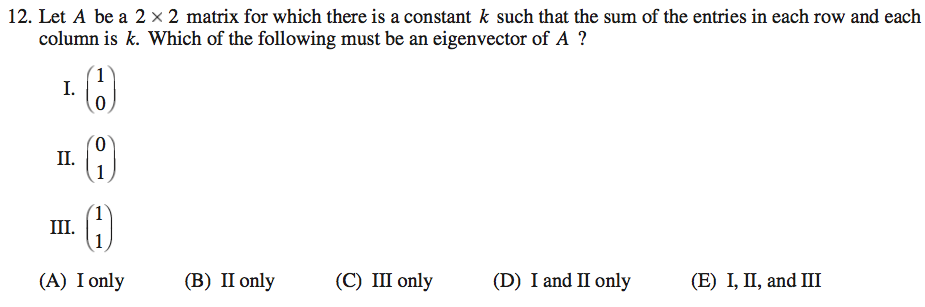
\includegraphics[scale=0.5]{0568_12}

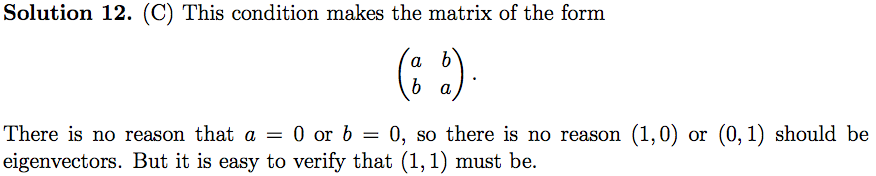
\includegraphics[scale=0.5]{0568_12s}

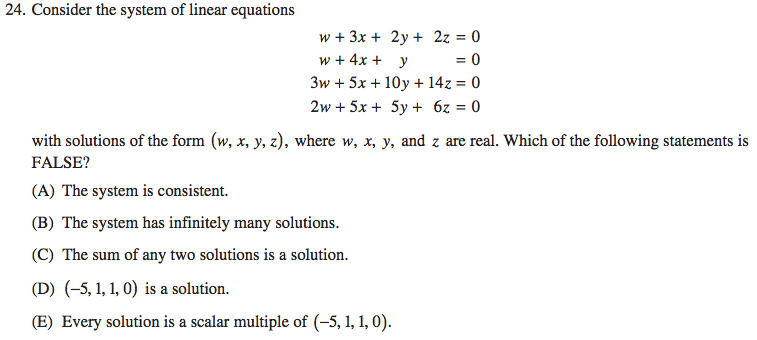
\includegraphics[scale=0.65]{1268_24}

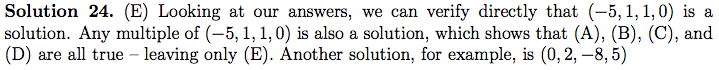
\includegraphics[scale=0.65]{1268_24s}

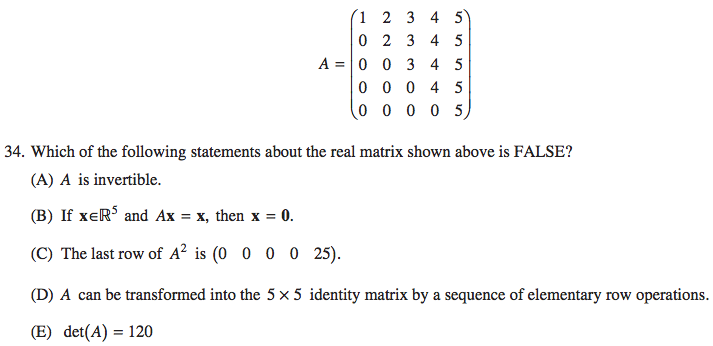
\includegraphics[scale=0.65]{1268_34}

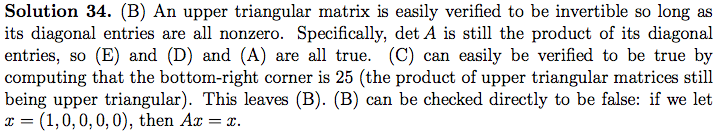
\includegraphics[scale=0.65]{1268_34s}

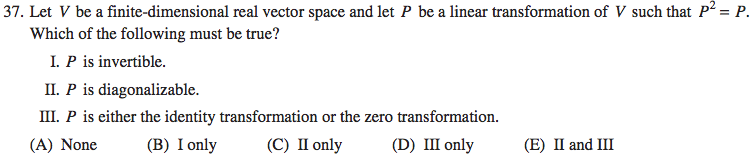
\includegraphics[scale=0.65]{1268_37}

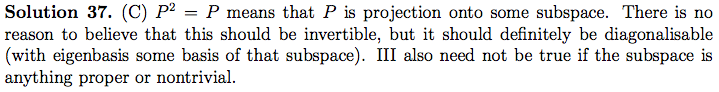
\includegraphics[scale=0.65]{1268_37s}

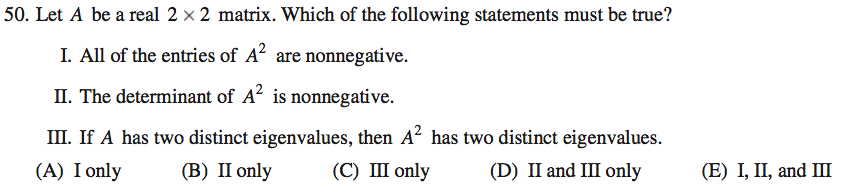
\includegraphics[scale=0.5]{0568_50}

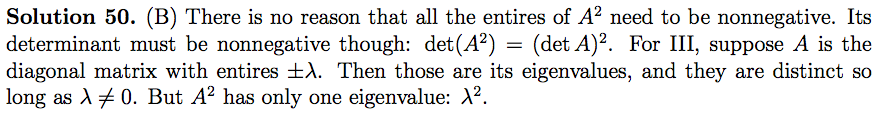
\includegraphics[scale=0.5]{0568_50s}

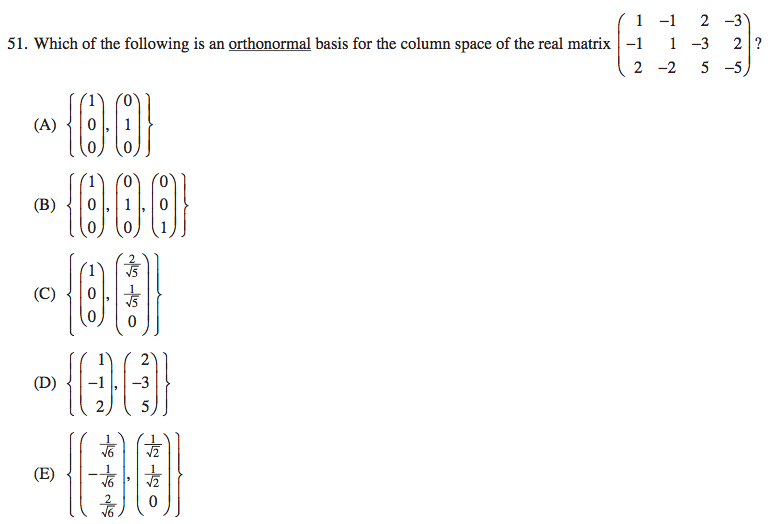
\includegraphics[scale=0.65]{1268_51}

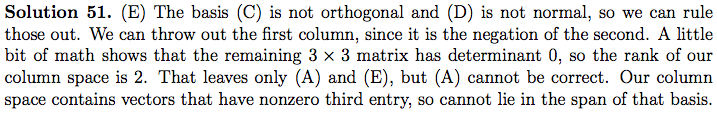
\includegraphics[scale=0.65]{1268_51s}

%%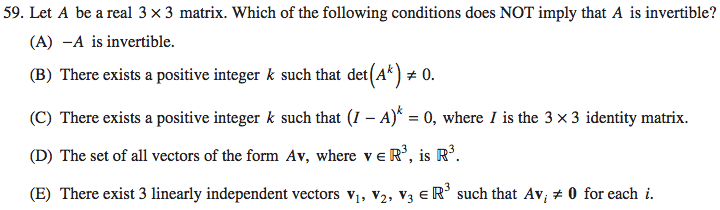
\includegraphics[scale=0.65]{1268_59}
%
%%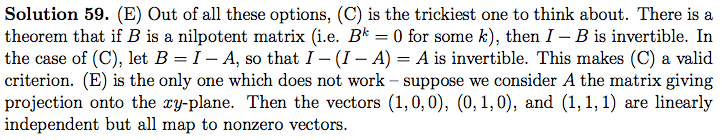
\includegraphics[scale=0.65]{1268_59s}

\pagebreak

% Calculus
\section{Calculus}

These notes include some screenshots from Wikipedia as well as from \textit{Calculus} by Gilbert Strang, available at \url{https://ocw.mit.edu/ans7870/resources/Strang/Edited/Calculus/Calculus.pdf}.

\subsection{List of common derivatives and integrals to know}

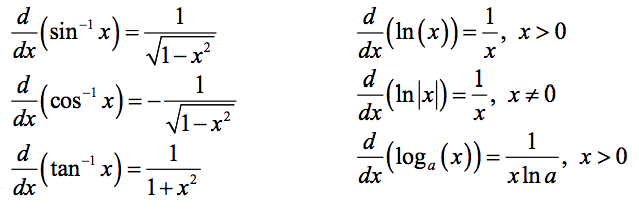
\includegraphics[scale=0.45]{derivatives}

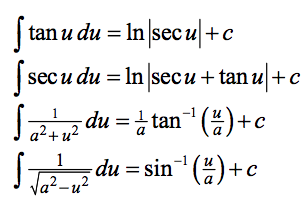
\includegraphics[scale=0.45]{integrals}

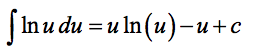
\includegraphics[scale=0.45]{integral_ln}

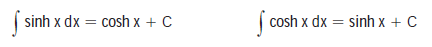
\includegraphics[scale=0.65]{integrals2}

\subsection{Optimizing functions of several variables}

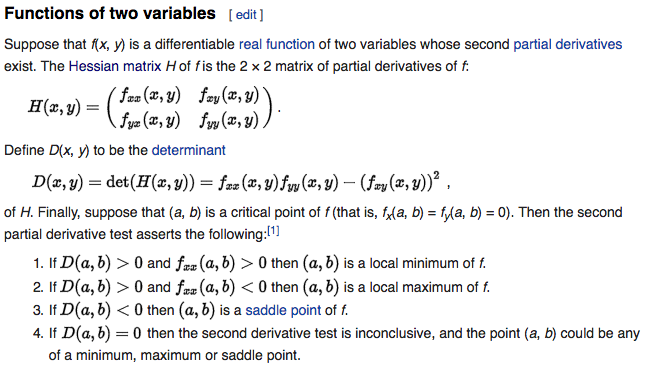
\includegraphics[scale=0.65]{hessian1}

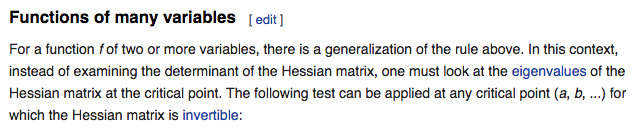
\includegraphics[scale=0.65]{hessian2}

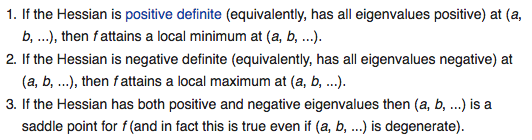
\includegraphics[scale=0.65]{hessian3}

\subsection{Lagrange Multipliers} \textbf{: to flesh out!} http://tutorial.math.lamar.edu/Classes/CalcIII/LagrangeMultipliers.aspx

\subsection{Line Integrals} (p. 555 of Strang book)

Suppose a force in two-dimensional space is given by \(\boldsymbol{F} = M\boldsymbol{i} + N \boldsymbol{j}\). Then the work done by this force on a particle moving along a curve \(C\) is given by

\[
W = \int_C \boldsymbol{F} \cdot \text{d}\boldsymbol{R} = \int_C M \text{d}x + N \text{d} y
\]

Along a curve in three-dimensional space the work done by a three-dimensional force \(\boldsymbol{F} = M\boldsymbol{i} + N \boldsymbol{j} + P \boldsymbol{j}\) is given by

\[
W = \int_C \boldsymbol{F} \cdot \boldsymbol{T} \text{d}s = \int_C \boldsymbol{F} \cdot \text{d}\boldsymbol{R} = \int_C M \text{d}x + N \text{d}y + P \text{d}z
\]

where the tangent vector \(\boldsymbol{T}\) is given by \[\boldsymbol{T} = \frac{\text{d}\boldsymbol{R}}{\text{d}s}\]

\textbf{Green's Theorem:} Suppose the region \(R\) is bounded by the simple closed piecewise smooth curve \(C\). Then an integral over \(R\) equals a line integral around \(C\):

\[
\oint_C \boldsymbol{F} \cdot \text{d}\boldsymbol{R} = \oint_C M \text{d}x + N \text{d}y = \int \int_R \bigg( \frac{\partial N}{\partial x} - \frac{\partial M}{\partial y} \bigg) \text{d}x \ \text{d}y
\]

\subsection{Miscellaneous}

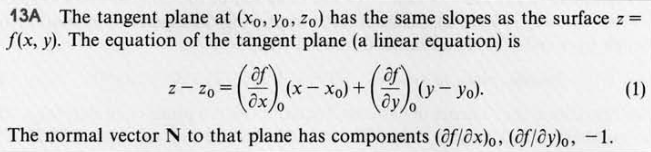
\includegraphics[scale=0.65]{tangent_plane}

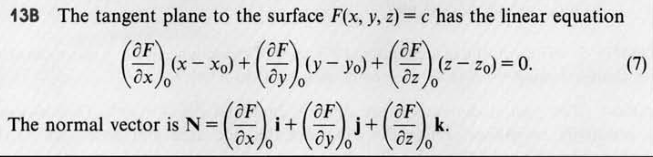
\includegraphics[scale=0.65]{tangent_plane2}

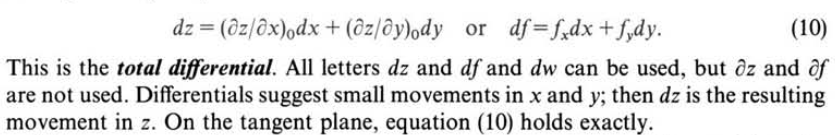
\includegraphics[scale=0.55]{total_differential}

The \textbf{directional derivative}, denoted \(D_v f(x, y)\), is a derivative of a multivariable function in the direction of a vector \(\boldsymbol{v}\). It is the scalar projection of the gradient onto \(\boldsymbol{v}\).

\[
D_v f(x, y) = \text{comp}_v \nabla f(x, y) = \frac{\nabla f(x, y) \cdot \boldsymbol{v}}{|\boldsymbol{v}|}
\]

\subsection{Practice Problems}

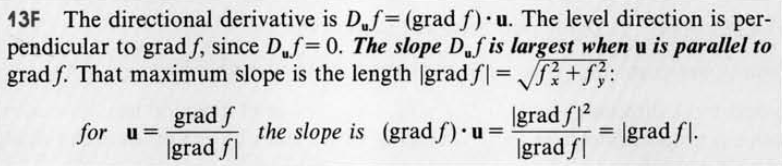
\includegraphics[scale=0.55]{gradient}

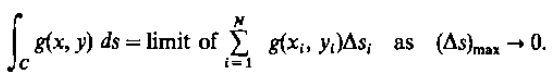
\includegraphics[scale=0.55]{line_int1}

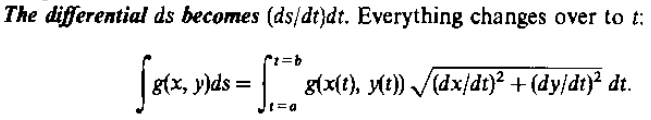
\includegraphics[scale=0.55]{line_int2}

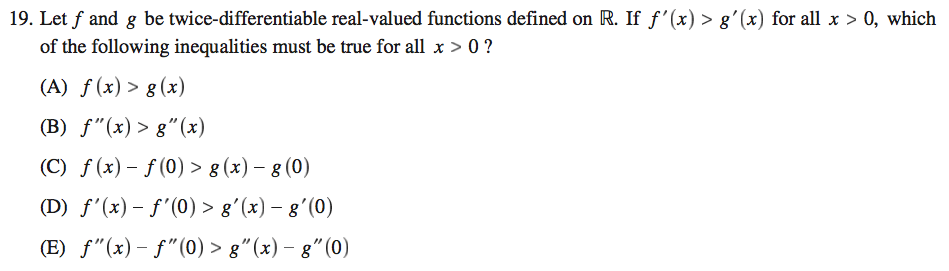
\includegraphics[scale=0.5]{0568_19}

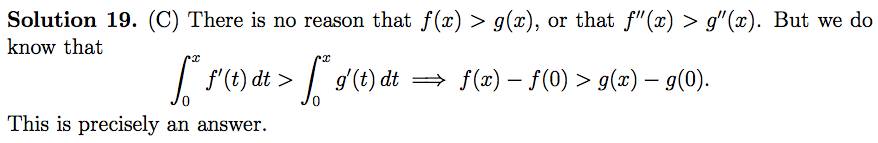
\includegraphics[scale=0.5]{0568_19s}

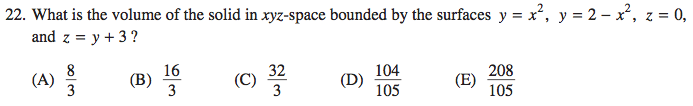
\includegraphics[scale=0.65]{1268_22}

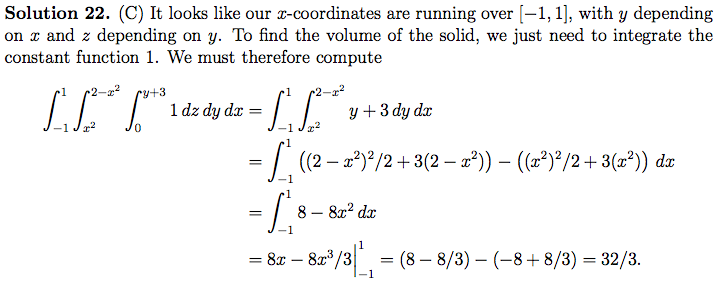
\includegraphics[scale=0.65]{1268_22s}

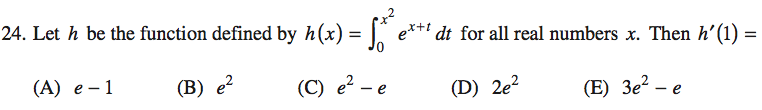
\includegraphics[scale=0.5]{0568_24}

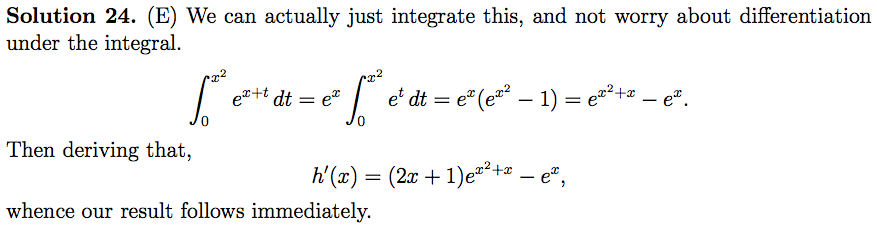
\includegraphics[scale=0.5]{0568_24s}

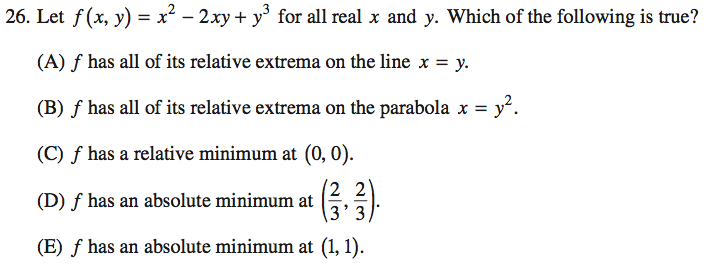
\includegraphics[scale=0.5]{0568_26}

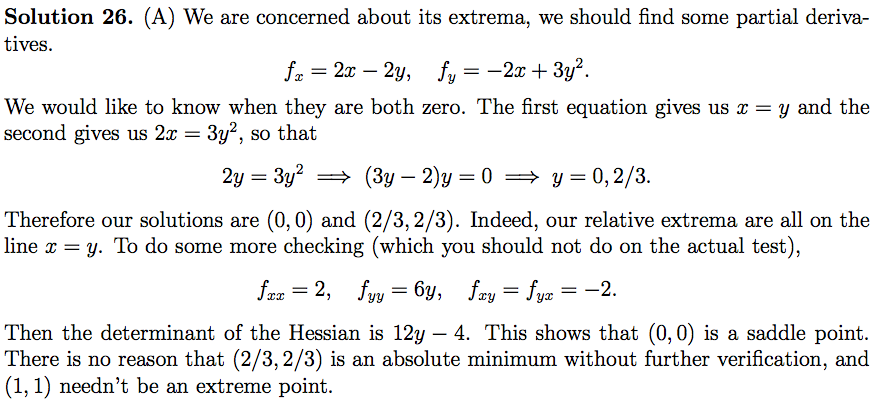
\includegraphics[scale=0.5]{0568_26s}

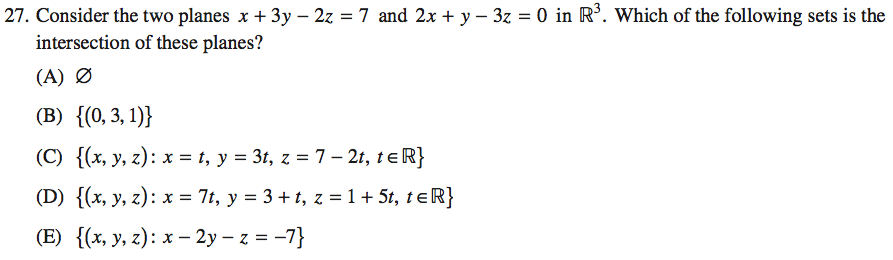
\includegraphics[scale=0.5]{0568_27}

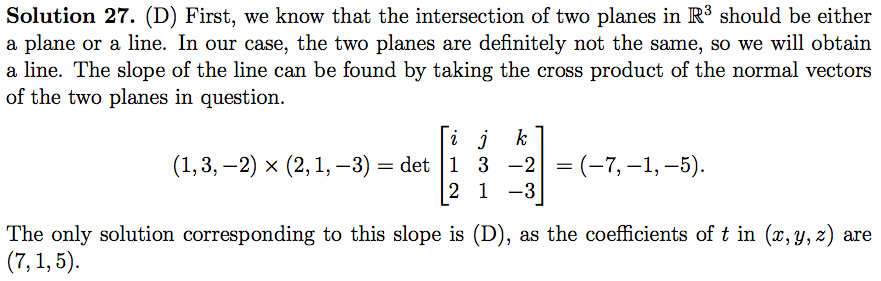
\includegraphics[scale=0.5]{0568_27s}

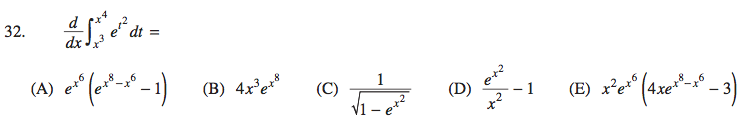
\includegraphics[scale=0.65]{1268_32}

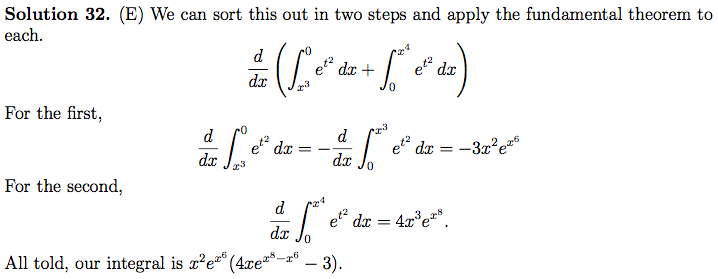
\includegraphics[scale=0.65]{1268_32s}

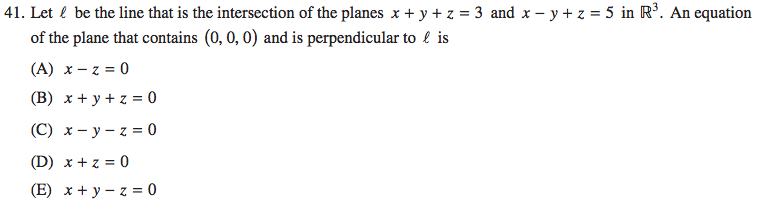
\includegraphics[scale=0.65]{1268_41}

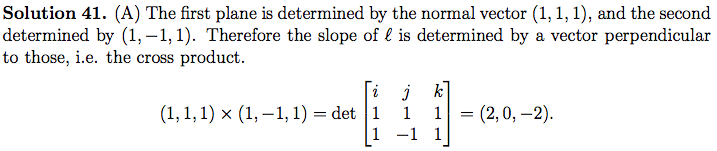
\includegraphics[scale=0.65]{1268_41s1}

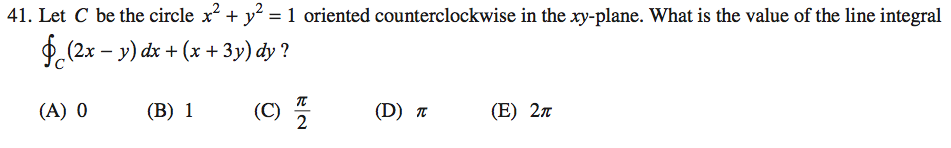
\includegraphics[scale=0.5]{0568_41}

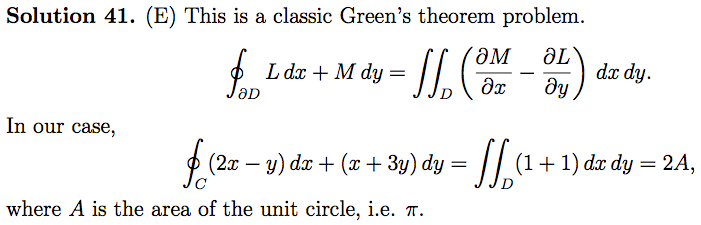
\includegraphics[scale=0.5]{0568_41s}

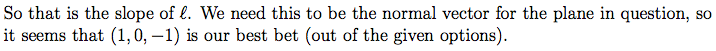
\includegraphics[scale=0.65]{1268_41s2}

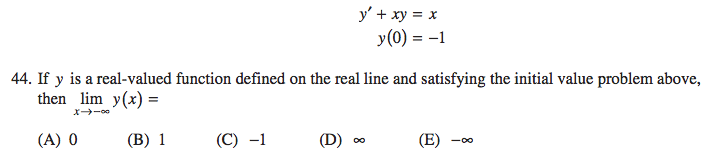
\includegraphics[scale=0.65]{1268_44}

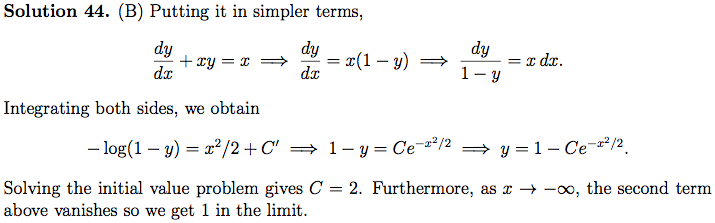
\includegraphics[scale=0.65]{1268_44s}


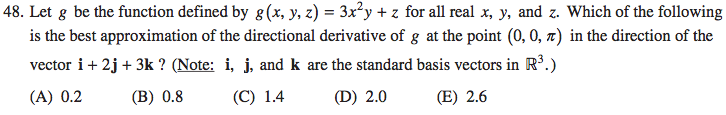
\includegraphics[scale=0.65]{1268_48}

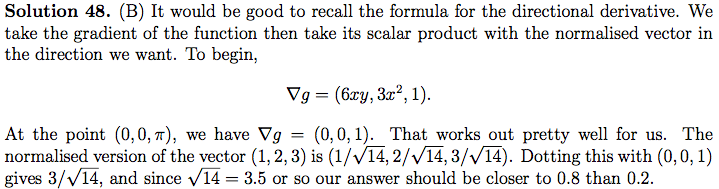
\includegraphics[scale=0.65]{1268_48s}

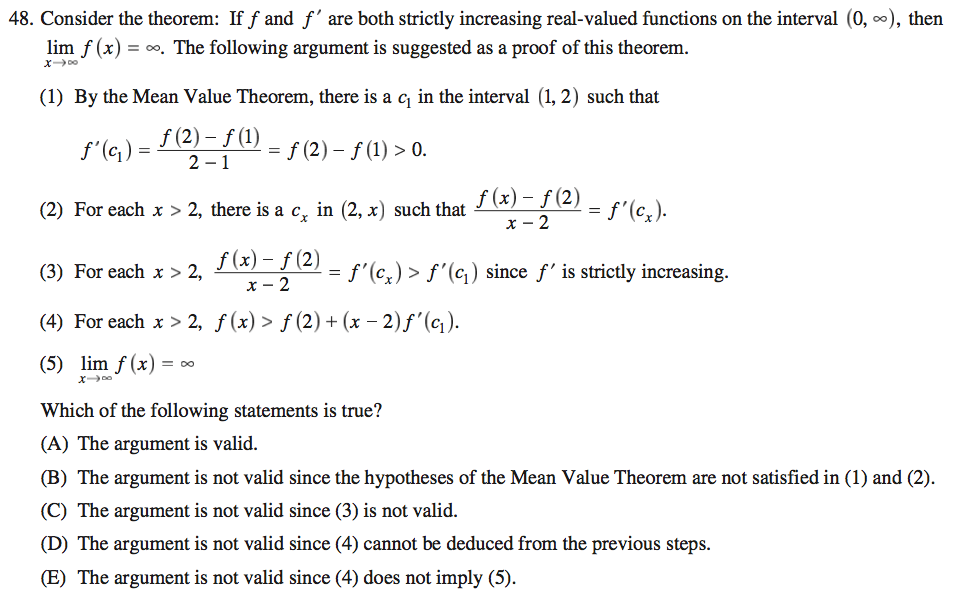
\includegraphics[scale=0.5]{0568_48}

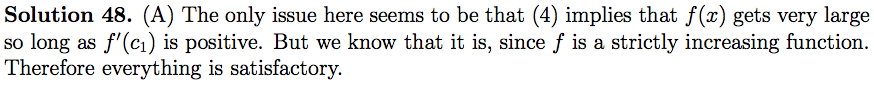
\includegraphics[scale=0.5]{0568_48s}

%\includegraphics[scale=0.65]{1268_53}

%\includegraphics[scale=0.65]{1268_53s}

%\includegraphics[scale=0.65]{1268_55}

%\includegraphics[scale=0.65]{1268_55s}

%\includegraphics[scale=0.65]{1268_56}
%
%\includegraphics[scale=0.65]{1268_56s1}

%\includegraphics[scale=0.65]{1268_56s2}

%\includegraphics[scale=0.65]{1268_64}
%
%\includegraphics[scale=0.65]{1268_64s}

\textbf{Line integrals chapter!} http://tutorial.math.lamar.edu/Classes/CalcIII/LineIntegralsIntro.aspx

\textbf{Surface inegrals chapter!} http://tutorial.math.lamar.edu/Classes/CalcIII/SurfaceIntegralsIntro.aspx

\pagebreak

% Differential Equations
\section{Differential Equations}

\includegraphics[scale=0.65]{1268_61}

\includegraphics[scale=0.65]{1268_61s}

\pagebreak

% Real Analysis
\section{Real Analysis}

These are my notes from Math 4650: Analysis I at Cal State LA.

%\textbf{Brush up on recent real analysis (especially open, closed, compact, etc)}

%Midterm 1
\subsection{Midterm 1}

% Homework 1
\subsubsection{Homework 1}

\textbf{Definition:} Let \(S \subseteq \mathbb{R}\). We say that \(S\) is \textbf{bounded from above} if \(\exists \ b \in \mathbb{R}\) where \[s \leq b \ \forall \ s \in S\]If this is the case, we call \(b\) an \textbf{upper bound} of \(S\).

If \(b \leq c \) for all upper bounds \(c\) of \(S\), we call \(b\) the \textbf{supremum} of \(S\): \(b = \sup(S)\).

We say that \(S\) is \textbf{bounded from below} if \(\exists \ a \in \mathbb{R}\) where \[s \geq a \ \forall \ s \in S\]If this is the case, we call \(a\) a \textbf{lower bound} of \(S\).

If \(a \geq d \) for all lower bounds \(d\) of \(S\), we call \(a\) the \textbf{infimum} of \(S\): \(a = \inf(S)\).

\textbf{Useful Sup/Inf Fact:} Let \(S \in \mathbb{R}\), \(S \neq \emptyset\). 

\begin{enumerate}[(1)]

\item Suppose \(S\) is bounded from above by an element \(b\). Then \(b = \sup(S) \iff \forall \ \epsilon >0 \ \exists \ x \in S\) with \[b - \epsilon < x \leq b\]

\item Suppose \(S\) is bounded from below by an element \(a\). Then \(a = \inf(S) \iff \forall \ \epsilon >0 \ \exists \ x \in S\) with \[a \leq x < a + \epsilon\]

\end{enumerate}

\textbf{Completeness Axiom}: Let \(S\) be a nonempty subset of \(\mathbb{R}\). If \(S\) is bounded from above, then \(\sup(S)\) exists. If \(S\) is bounded from below, then \(\inf(S)\) exists.

%\[
%|x - y| < \epsilon \iff y - \epsilon < x < y + \epsilon
%\]

\textbf{Facts about absolute value:}

\begin{enumerate}[(1)]

\item \(|x-y| < \epsilon \iff y - \epsilon < x < y + \epsilon\) (proof: in notes 08/23)

\item \(|ab| = |a||b|\) (proof: 7(c) in Homework 1)

\item Let \(\epsilon >0\). Then \(|a| < \epsilon \iff -\epsilon < a < \epsilon\). (Proof: follows from (1) if \(x = a\), \(y = 0\).)

\item \(-|a| \leq a \leq |a|\) (proof: Follows from (1) if \(x = a\), \(y = 0\), \(\epsilon = |a|\).)

\item \textbf{Triangle Inequality:} \(|a + b| \leq |a| + |b|\) (Proof in notes 08/23)

\item \(|\ |a| - |b| \ | \leq |a - b|\) (Proof: 7(d) in Homework 1)

\item \textbf{Triangle Inequality:} \(|a - b| \leq |a| + |b|\) (Proof: follows from (5), let \(b = -b\).)

\item If \(a < x < b\) and \(a < y < b\) then \(|x - y| < b - a\). (Proof: 7(a) in Homework 1)

\item \(|a - b| = |b - a|\) (Proof: 7(b) in Homework 1.)

\end{enumerate}

% Homework 2
\subsubsection{Homework 2}

\textbf{Definition:} A sequence \((a_n)\) of real numbers is said to \textbf{converge} to a \textbf{limit} \(L \in \mathbb{R}\) if \(\forall \ \epsilon > 0 \ \exists \ N > 0 \) where

\[
n \geq N \implies |a_n - L| < \epsilon
\]

We say that \((a_n)\) \textbf{diverges} if it does not converge.

\textbf{Definition:} A sequence \((a_n)\) of real numbers is \textbf{bounded} if \(\exists \ M > 0\) where \(\forall \ n \in \mathbb{N}\) \[\ |a_n| \leq M \]

\textbf{Theorem.} If \((a_n)\) converges then \((a_n)\) is bounded.

\textbf{Definition:} Let \((a_n)\) be a sequence of real numbers. We say that \((a_n)\) is a \textbf{Cauchy sequence} if \(\forall \ \epsilon > 0 \ \exists \ N\) where

\[
n, m \geq N \implies |a_n - a_m| < \epsilon
\]

\textbf{Theorem.} \((a_n)\) is Cauchy if and only if \((a_n)\) converges.

\textbf{Corollary.} If \((a_n)\) is Cauchy then \((a_n)\) is bounded.

\pagebreak

% Midterm 2
\subsection{Midterm 2}

% Homework 3
\subsubsection{Homework 3}

\textbf{Limits of functions at infinity.} Let \(f\) be a real-valued function defined on some set \(D\) where \(D\) contains an interval of the form \((a, \infty)\). Let \(L \in \mathbb{R}\). We say \[\lim_{x \to \infty} f(x) = L\]if \(\forall \ \epsilon >0 \ \exists \ N \in \mathbb{R}\) where

\[
x \geq N \implies |f(x) - L| < \epsilon
\]

\textbf{Definition:} Let \(D \subseteq \mathbb{R}\). Let \(a \in \mathbb{R}\). We say that \(a\) is a \textbf{limit point} (or ``cluster point," or ``accumulation point") of \(D\) if \(\forall \ \delta > 0 \ \exists \ x \in D\) where

\[
x \neq a \text{ and } |x - a| < \delta
\]

(Note that \(a\) may or may not be contained in \(D\).)

\textbf{Limit of a function at \(a\)}: Let \(D \subseteq \mathbb{R}\) and \(f:d \to \mathbb{R}\). Let \(a\) be a limit point of \(D\). Let \(x \in D\). We say that \(f\) has a \textit{limit as \(x\) tends to \(a\)} if \(\exists \ L \in \mathbb{R}\) where \(\forall \ \epsilon > 0 \ \exists \ \delta > 0 \) such that

\[
0 < |x - a| < \delta \implies |f(x) - L| < \epsilon
\]

and we write \[\lim_{x \to a} f(x) = L\]

\textbf{Properties of Limits:} Let \(D \in \mathbb{R}\) and let \(a\) be a limit point of \(D\). Suppose \(f:D \to \mathbb{R}\) and \(g: D \to \mathbb{R}\). Let \(\alpha \in \mathbb{R}\).

\begin{enumerate}[(1)]

\item If \(\lim_{x \to a} f(x) = L\) and \(\lim_{x \to a} g(x) = M\) then

\begin{enumerate}[(a)]

\item \[\lim_{x \to a} \alpha = \alpha\]

\item \[\lim_{x \to a} [f(x) + g(x)] = L + M\]

\item \[\lim_{x \to a} [f(x) - g(x)] = L - M\]

\item \[\lim_{x \to a} [f(x) \cdot g(x)] = L \cdot M\]

\item \[\lim_{x \to a} [\alpha \cdot f(x)] = \alpha \cdot L\]

\end{enumerate}

\item If \(h:D \to \mathbb{R}\) and \(h(x) \neq 0 \ \forall \ x \in D\) and \(\lim_{x \to a} h(x) = H \neq 0\), then

\[
\lim_{x \to a} \frac{1}{h(x)} = \frac{1}{H}
\]

Note that properties (2) and (1)(d) combined imply

\[
\lim_{x \to a} \frac{f(x)}{h(x)} = \frac{L}{H}
\]

\end{enumerate}

% Homework 4
\subsubsection{Homework 4}

\textbf{Continuity:} Let \(D \subseteq \mathbb{R}\) and \(f:D \to \mathbb{R}\) and \(a \in D\). Then \(f\) is \textbf{continuous} at \(a\) if \(\lim_{x \to a} f(x)\) exists and 

\[
\lim_{x \to a} f(x) = f(a)
\]

(Note: if \(f\) is continuous at \(a\), then we can say \(\forall \ \epsilon > 0 \ \exists \ \delta > 0 \) such that

\[
|x - a| < \delta \implies |f(x) - L| < \epsilon
\]

that is, we don't need to say \(0 < |x - a| < \delta\)).

If \(B \subseteq D\), then \(f\) is \textbf{continuous on B} if \(f\) is continuous at every \(b \in B\).

\textbf{Intermediate Value Theorem:} Let \(f\) be continuous on \([a, b]\) and suppose \(f(a) < f(b)\). \(\forall \ d\) such that \[f(a) < d < f(b)\]  \(\exists \ c \in \mathbb{R}\) where \[a < c < b, \ f(c) = d\]

\pagebreak

% Final
\subsection{Final}

% Homework 5
\subsubsection{Homework 5}

\textbf{Definition:} Let \(S \subseteq \mathbb{R}\). We say \(x \in \mathbb{R}\) is an \textbf{interior point} of \(S\) if there exists an open interval \((a, b)\) where \[x \in (a, b) \text{ and } (a, b) \subseteq S\]

\textbf{Open sets:} Let \(S \subseteq \mathbb{R}\). We say \(S\) is \textbf{open} if every \(x \in S\) is an interior point of \(S\).

\textbf{Closed sets:} Let \(S \subseteq \mathbb{R}\). We say \(S\) is \textbf{closed} if \(\mathbb{R} \setminus S\) is open.

\textbf{Theorem.} A set is closed if and only if it contains all of its limit points.

\textbf{Facts about open and closed sets:} Suppose \(a, b \in \mathbb{R}\). Then

\begin{itemize}

\item \((a, \infty)\) is open (Proof: Homework 5 problem 5b).

\item \((-\infty, b)\) is open (Proof: Homework 5 problem 5a).

\item \((a, b)\) is open (Proof: class notes).

\item If \(a < b\), then \([a, b]\) is closed (Proof: Homework 5 problem 5c).

\item If \(A\) and \(B\) are open, then \(A \cup B\) and \(A \cap B\) are open (Proof: Homework 5 problem 3).

\item If \(A\) and \(B\) are closed, then \(A \cup B\) and \(A \cap B\) are closed (Proof: Homework 5 problem 4).

\item \(\mathbb{R}\) is open (Proof: Homework 5 problem 1) and closed (Proof: \(\mathbb{R} \setminus \mathbb{R} = \emptyset\) is open).

\item \(\emptyset\) is open (Proof: Homework 5 problem 2) and closed (Proof: \(\mathbb{R} \setminus \emptyset = \mathbb{R}\) is open).

\end{itemize}

\textbf{Definition:} Let \(S \subseteq \mathbb{R}\). An \textbf{open cover} of \(S\) is a collection \(X = \{\mathcal{O}_\alpha \ | \ \alpha \in I \} \) where each set \(\mathcal{O}_\alpha\) is an open subset of \(\mathbb{R}\) such that

\[
S \subseteq \bigcup_{\alpha \in I} \mathcal{O}_\alpha
\]

(Here \(I\) is some set that indexes the \(\mathcal{O}_\alpha\)).

If \(X' \subseteq X\) such that \[S \subseteq  \bigcup_{\mathcal{O}_\alpha \in X'} \mathcal{O}_\alpha\]then \(X'\) is called a \textbf{subcover} of \(S\) contained in \(X\). In addition, if \(X'\) is finite then we call \(X'\) a \textbf{finite subcover} of \(S\) contained in \(X\).

\textbf{Compactness:} Let \(S \subseteq \mathbb{R}\). We say that \(S\) is \textbf{compact} if every open cover of \(S\) contains a finite subcover. 

\textbf{Definition:} Let \(S \subseteq \mathbb{R}\). We say that \(S\) is \textbf{bounded} if \(\exists \ M > 0\) where \(S \subseteq [-M, M]\).

Note: \(S\) is bounded if and only if \(|s| \leq M\  \forall \ s \in S \).

\textbf{Heine-Borel Theorem.} Let \(S \subseteq \mathbb{R}\). \(S\) is compact if and only if \(S\) is closed and bounded.

%\pagebreak

\textbf{Theorem.} Let \(f: D \to \mathbb{R}\) be continuous on \(D\). If \(X \subseteq D\) and \(X\) is compact (closed and bounded), then

\[
f(\bar{x}) = \{f(x) \ | \ x \in X\}
\]

is compact (closed and bounded).

\textbf{Corollary:} Suppose \(f: D \to \mathbb{R}\) where \(D\) is closed and bounded. Then there exists \(a, b \in D\) where \(f(a)\) is the min of \(f\) on \(D\) and \(f(b)\) is the max of \(f\) on \(D\).

% Homework 6
\subsubsection{Homework 6}

\textbf{Uniform Continuity:} Let \(D \subseteq \mathbb{R}\) and let \(f: D \to \mathbb{R}\). We say that \(f\) is \textbf{uniformly continuous} on \(D\) if \(\forall \ \epsilon > 0 \ \exists \ \delta > 0\) where

\[
x, y \in D \text{ and } 0 < |x - y| < \delta \implies |f(x) - f(y)| < \epsilon
\]

\textbf{Uniform continuity implies continuity.} Suppose \(f:D \to \mathbb{R}\) where \(D \subseteq \mathbb{R}\). If \(f\) is uniformly continuous on \(D\), then \(f\) is continuous at every \(a \in D\).


%\includegraphics[scale=0.65]{1268_36}
%
%\includegraphics[scale=0.65]{1268_36s}

\includegraphics[scale=0.5]{0568_38}

\includegraphics[scale=0.5]{0568_38s}

\includegraphics[scale=0.65]{1268_47}

\includegraphics[scale=0.65]{1268_47s}

\includegraphics[scale=0.65]{1268_57}

\includegraphics[scale=0.65]{1268_57s}

\includegraphics[scale=0.65]{1268_60}

\includegraphics[scale=0.65]{1268_60s}

\includegraphics[scale=0.65]{1268_63}

\includegraphics[scale=0.65]{1268_63s}

\pagebreak

% Probability

\section{Probability}

These are my notes from taking Math 505A at USC and the textbook \textit{Probability and Random Processes} (Grimmet and Stirkazer) 3rd edition.

\subsection{To Know for Math 505A Midterm 1 (Discrete Random Variables)}

\subsubsection{Definitions}

The \textbf{probability mass function} of a discrete random variable \(X\) is the function \(f: \mathbb{R} \to [0,1]\) given by \(f(x) = \Pr(X = x)\).

The \textbf{(cumulative) distribution function} of a discrete random variable \(F\) is given by \[F(x) = \sum_{i:x_i \leq x} f(x_i)\]

The \textbf{joint probability mass function} \(f: \mathbb{R}^2 \to [0, 1]\) of two discrete random variables \(X\) and \(Y\) is given by

\[
f(x, y) = \Pr(X = x \cap Y = y)
\]

The \textbf{joint distribution function} \(F: \mathbb{R}^2 \to [0, 1]\) is given by

\[
F(x, y) = \Pr(X \leq x \cap Y \leq y)
\]

If \(\Pr(B) > 0\) then the \textbf{conditional probability} that \(A\) occurs given that \(B\) occurs is defined to be

\[
\Pr(A \mid B) = \frac{\Pr(A \cap B)}{\Pr(B)}
\]

If \(X\) is a random variable and \(Y\) is a discrete random variable taking on values \(y_1, y_2, \ldots, y_n\), then \(\Pr(X) = \sum_i \Pr(X \mid Y = y_i) \cdot \Pr(Y = y_i)\). (Can be used to prove independence.)

Two random variables \(X\) and \(Y\) are \textbf{uncorrelated} if \(\E(XY) = \E(X) \E(Y)\). Two random variables are uncorrelated if and only if their covariance \(\Cov(X, Y) = \E \big[(X - \E(X))(Y - \E(Y))\big] = \E(XY) - \E(X)\E(Y)\)  equals 0. If \(X\) and \(Y\) are independent then they are uncorrelated.

Two random variables \(X\) and \(Y\) are \textbf{independent} if and only if \(\Pr(X \cap Y) = \Pr(X) \Pr(Y)\).

\textbf{Thereom.} If \(X\) and \(Y\) are independent and \(g, h: \mathbb{R} \to \mathbb{R}\), then \(g(X)\) and \(h(Y)\) are also independent.

\subsubsection{Conditioning}

The \textbf{conditional distribution function} of \(Y\) given \(X = x\), written \(F_{Y\mid X}( \cdot \mid x)\), is defined by

\[
F_{Y\mid X}( y \mid x) = \Pr(Y \leq y \mid X = x)
\]

The \textbf{conditional probability mass function} of \(Y\) given \(X = x\), written \(f_{Y\mid X}( \cdot \mid x)\), is defined by

\[
f_{Y\mid X}( y \mid x) = \Pr(Y = y \mid X = x)
\]

\textbf{Iterated expecations:} 

\begin{itemize}

\item \(\E\big[ \E(Y \mid X) \big] = \E(Y)\)

\item \(\E \big[ (X \mid Y) \mid Z \big] = \E(X \mid Y)\)

\item \( \E(E(XY \mid Y)) = \E(Y \E(X \mid Y))\)

\end{itemize}

\textbf{Conditional Variance:} \(\Var(X \mid Y) = \E\big[ (X - \E(X \mid Y))^2   \mid Y\big]\)

\subsubsection{Odds and Ends}

\textbf{Inclusion-Exclusion Principle:}

\[
\Pr \bigg( \bigcup_{i=1}^n A_i \bigg) = \sum_{k=1}^n (-1)^{k+1} \bigg( \sum_{1 \leq i_1 < \ldots < i_k \leq m} \Pr \big(A_{i1} \cap \ldots \cap A_{ik} \big) \bigg)
\]

\[
\left| \bigcup_{i=1}^n A_i \right| = \sum_{k=1}^n (-1)^{k+1} \bigg( \sum_{1 \leq i_1 < \ldots < i_k \leq m} \left| A_{i1} \cap \ldots \cap A_{ik} \right| \bigg)
\]

\textbf{Sums of random variables.} If \(X\) and \(Y\) are independent then

\[
\Pr(X + Y = z) = f_{X +Y}(z) = \sum_x f_X(x) f_Y(z-x) = \sum_y f_X(z - y) f_Y(y)
\]

\textbf{Variance-Covariance Expansion.} Let \(X_1, \ldots, X_n\) be random variables. If \(\E \left|X_k \right|^2 < \infty\), then 

\[
\Var(X_1 + \ldots + X_n) = \sum_k \Var(X_k) + \sum_{k \neq m} \sum_m \Cov(X_k, X_m)
\]

\subsubsection{Methods for Calculating Quantities}

\begin{itemize}

\item Expectation

\begin{itemize}

\item Definition: \(\E(X) = \sum_x x \Pr(X = x)\)\

\item Useful theorems: \(\E(aX + bY) = a \E(X) + b \E(Y)\); if \(X \geq 0\) then \(\E(X) \geq 0\).

\item \textbf{Law of the Unconscious Statistician:} If \(X\) has mass function \(f\), and \(g: \mathbb{R} \to \mathbb{R}\), then 

\[
\E(g(X)) = \sum_x g(x) f(x)
\]

\item Expectation is a linear operator: \( \E \big(\sum_i X_i \big) = \sum_i \E(X_i)\)



\end{itemize}

\item Variance

\begin{itemize}

\item Definition: \( \Var(X) = \E(X - \E(X))^2\)

\item Useful reformulation: \(\Var(X) = \E(X^2) - \E(X)^2\)

\item Useful theorems: \(\Var(aX) = a^2 \Var(X)\), \(\Var(X + Y) = \Var(X) + \Var(Y) + 2 \Cov(X, Y)\), \(\Var(aX \pm bY) = a^2\Var(X) + b^2\Var(Y) \pm 2ab \Cov(X, Y)\)

\item \textbf{Total variance:} \( \Var(X) = \Var \big( \E(X \mid Y) \big) + \E \big( \Var(X \mid Y) \big) \)

\end{itemize}

\item Covariance

\begin{itemize}

\item Definition: \( \Cov(X, Y ) = \E \big[ (X - \E(X))(Y - \E(Y))\big] \)

\item Useful reformulation: \(\Cov(X) = \E(XY) - \E(X)\E(Y)\)

\end{itemize}

\end{itemize}

\subsubsection{Discrete Random Variable Distributions}

\textbf{Binomial}: \(\operatorname{Binomial}(n, p)\) (sum of \(n\) Bernoulli random variables)

\begin{itemize}

\item Mass function: \(\Pr(X = k) = \binom{n}{k}p^k(1-p)^{n-k}  \)

\item Distribution: \(\Pr(X \leq k) = \sum_{i=0}^k \binom{n}{i}p^i(1-p)^{n-i} \)

\item Expectation: \(\E(X) = np \)

\item Variance: \(\Var(X) = np(1-p) \)

\end{itemize}

\textbf{Poisson}:  \(\operatorname{Poisson}(\lambda)\): an approximation of the binomial distribution for n very large, p very small, \(np \to \lambda \in (0, \infty)\).

\begin{itemize}

\item Mass function: \[\Pr(X = k) =  \frac{e^{-\lambda}\lambda^k}{k!} \]

\item Distribution: \(\Pr(X \leq k) = \sum_{i=0}^k  \frac{e^{-\lambda}\lambda^i}{i!}  \)

\item Expectation: \(\E(X) = \lambda \) (derive from basic definitions)

\item Variance: \(\Var(X) = \lambda\)

\end{itemize}

\textbf{Geometric}:  \(\operatorname{G}_1(p)\): the number of Bernoulli trials before the first success.

\begin{itemize}

\item Mass function: \(\Pr(X = k) = p(1-p)^{k-1} \)

\item Distribution: \(\Pr(X \leq k) = \sum_{i=1}^k p(1-p)^{k-1}  \)

\item Expectation: \(\E(X) = 1/p \)

\item Variance: \(\Var(X) = (1-p)/p^2\)

\end{itemize}


\textbf{Negative binomial}: \( \operatorname{NB}(r, p)\): The number of Bernoulli trials required for \(r\) successes. (Can be derived as the sum of \(r\) identically distributed geometric random variables.)

\begin{itemize}

\item Mass function: \(\Pr(X = k) =  \binom{k-1}{r-1} p^r (1-p)^{k-r}\)

\item Distribution: \(\Pr(X \leq k) = \sum_{i=r}^k \binom{i-1}{r-1} p^r (1-p)^{i-r} \)

\item Expectation: \(\E(X) = \)

\item Variance: \(\Var(X) = \)

\end{itemize}


\textbf{Hypergeometric}: \( \operatorname{Hypergeometric}(N, M, K)\): When drawing a sample of size \(K\) from a group of \(N\) items, \(M\) of which are special, the number of special items retrieved.

\begin{itemize}

\item Mass function: \[\Pr(X = k) = \frac{\binom{M}{k} \binom{N-M}{K-k}}{\binom{N}{K}} \]

\item Distribution: \[\Pr(X \leq k) = \sum_{i=0}^k \frac{\binom{M}{i} \binom{N-M}{K-i}}{\binom{N}{K}}  \]

\item Expectation: \(\E(X) = \) (find by indicator method)

\includegraphics[scale=0.1]{prob_hypergeometric}

\item Variance: \(\Var(X) = \) (find by indicator method)

\end{itemize}


\subsubsection{Indicator Method}

If \(\boldsymbol{1}_{A_k}\) is an indicator then

\[
\Cov(\boldsymbol{1}_{A_k}, \boldsymbol{1}_{A_m}) = \E(\boldsymbol{1}_{A_k} \boldsymbol{1}_{A_m}) - \E(\boldsymbol{1}_{A_k}) \E(\boldsymbol{1}_{A_m}) = \Pr(A_k \cap A_m) - \Pr(A_k) \Pr(A_m)
\]

\[
\Var(\boldsymbol{1}_{A_k} ) = \E(\boldsymbol{1}_{A_k} ^2) = \E(\boldsymbol{1}_{A_k} )^2 = \Pr(A_k) - (\Pr(A_k))^2
\]

\(X\) is independent of \(Y\) if and only if \(X\) is independent of \(\boldsymbol{1}_A\), \(A \in Y\).

Example problems: 505A Homework 3 problem 9(a)

Worked examples in p. 56 - 59 of Grimmet and Stirkazer 3rd edition.

\subsubsection{Linear transformations of random variables}

\subsubsection{Poisson Paradigm (Poisson approximation for indicator method)}

(Theorem 9, p. 129.) Let \(A_i\) be an event. If \(X = \sum_{i=1}^m \boldsymbol{1}_{A_i}\) where \(\boldsymbol{1}_{A_i}\) is an indicator variable for \(A_i\), and the \(A_i\) are only weakly dependent on each other, then 

\[
\text{As } m \to \infty, \ \ X \sim \operatorname{Poisson}(\E(X))
\]

More specifically, let \(B_i\) be \(n\) independent Bernoulli random variables with probabilities \(p_i\). If \(Y = \sum_{i=1}^n B_i\) then 

\[
\text{As } n \to \infty, \ \ Y \sim \operatorname{Poisson} \bigg(\E \bigg(\sum_i B_i \bigg) \bigg) = \operatorname{Poisson}\bigg(\sum_i \E B_i \bigg) = \operatorname{Poisson}\bigg(\sum_i p_i \bigg) 
\]

\subsubsection{Asymptotic Distributions}

\[
e^x = \lim_{n \to \infty} \bigg( 1 + \frac{x}{n}\bigg)^n
\]

\textbf{Stirling's Formula}: 

\[
n! \approx n^ne^{-n} \sqrt{2\pi n}
\]

%%%%%%%% Example Problems That Will Likely Appear on Midterm %%%%%%%%%%%%%
\subsection{Worked problems}

\subsubsection{Example Problems That Will Likely Appear on Midterm}

\textbf{Fall 2011 Problem 1 (same as HW1 problem 5; similar to HW3 problem 2(5); likely to be question 1 on the midterm.)} True or false: if \(A\) and \(B\) are events such that \( 0 < \Pr(A) < 1\) and \(\Pr(B \mid A) = \Pr(B \mid A^c)\), then \(A\) and \(B\) are independent.

\textbf{Solution.} \(A\) and \(B\) are independent if and only if 

\[
\Pr(A \cap B) = \Pr(A)\cdot\Pr(B)
\]

We know that \[ \Pr(B) = \Pr(B|A)\cdot \Pr(A) + \Pr(B|A^c)\cdot\Pr(A^c)  \]

\[
= \Pr(B|A)\cdot \Pr(A) + \Pr(B|A)\cdot (1 - \Pr(A)) = \Pr(B|A)\cdot \Pr(A) + \Pr(B|A) - \Pr(B|A)\cdot \Pr(A) 
\]

\[
= \Pr(B|A)
\]

Also, we know that since \(\Pr(A) \neq 0\),

\[
\Pr(B|A) = \frac{\Pr(A \cap B)}{\Pr(A)} 
\]

Per above \(\Pr(B|A) = \Pr(B)\), so we have

\[
\Pr(B) = \frac{\Pr(A \cap B)}{\Pr(A)} 
\]

\[
\Pr(A \cap B)= \Pr(A) \cdot \Pr(B)
\]

which is what we were trying to prove. So the answer is \(\boxed{\text{true.}}\)

\textbf{Similar problem: HW3 Problem 2(5).} Verify: \(\E(X \mid Y) = \E(X)\) if \(X\) and \(Y\) are independent.

\textbf{Solution.} \(X\) and \(Y\) are independent if and only if

\[
\Pr(X \cap Y) = \Pr(X)\cdot\Pr(Y) \iff \Pr(X = x \cap Y = y) = \Pr(X = x) \Pr(Y = y)
\]

\[
\iff \Pr(X = x \mid Y = y) \cdot \Pr(Y = y) =  \Pr(X = x) \Pr(Y = y) \iff \Pr(X = x \mid Y = y) = \Pr(X = x)
\]

\[
\implies E(X \mid Y) = \sum_x x \cdot \Pr(X = x \mid Y = y ) = \sum_x x \cdot \Pr(X = x ) = \E(X)
\]


\textbf{Fall 2014 Problem 1 (likely to be question 2 on the midterm).} Let \(A\) and \(B\) be two events with \(0 < \Pr(A) < 1, \ 0 < \Pr(B) < 1\). Define the random variables \(\xi = \xi(\omega)\) and \(\eta = \eta(\omega)\) by

\[
\xi(\omega) = \begin{cases} 
      5 & \text{ if } \omega \in A \\
      -7 &  \text{ if } \omega \notin A 
   \end{cases}, \ \ \ \ \eta(\omega) = \begin{cases} 
      2 & \text{ if } \omega \in B \\
      3 &  \text{ if } \omega \notin B 
   \end{cases}
\]

True or false: the events \(A\) and \(B\) are independent if and only if the random variables \(\xi\) and \(\eta\) are uncorrelated?

\textbf{Solution.} (\(\implies\)) Suppose \(A\) and \(B\) are independent. Then \(\xi\) and \(\eta\) are uncorrelated if and only if \(\E(\xi \eta ) = \E(\xi) \E(\eta)\). We can write \(\xi = 5 \cdot \boldsymbol{1}_A - 7 \cdot \boldsymbol{1}_{A^c}\) and \(\eta = 2 \cdot \boldsymbol{1}_B + 3 \cdot \boldsymbol{1}_{B^c}\). So we have

\[
\xi \eta = (5 \cdot \boldsymbol{1}_A - 7 \cdot \boldsymbol{1}_{A^c})(2 \cdot \boldsymbol{1}_B + 3 \cdot \boldsymbol{1}_{B^c}) = 10 \cdot \boldsymbol{1}_{A \cap B} +15 \cdot \boldsymbol{1}_{A \cap B^c} - 14 \cdot \boldsymbol{1}_{A^c \cap B} - 21 \cdot \boldsymbol{1}_{A^c \cap B^c}
\]

\[
\implies \E(\xi \eta ) = 10 \Pr(A \cap B) +15\Pr(A \cap B^c) - 14 \Pr(A^c \cap B) - 21\Pr(A^c \cap B^c)
\]

Then

\[
\E(\xi) \E(\eta) = (5 \Pr(A) - 7 \Pr(A^c))(2 \Pr(B) + 3 \Pr(B^c)) 
\]

\[
= 10\Pr(A \cap B) + 15 \Pr(A \cap B^c) - 14 \Pr(A^c \cap B) - 21 \Pr(A^c \cap B^c) = \E(\xi \eta )
\]

where the second-to-last step follows from the independence of \(A\) and \(B\). Therefore \(\eta\) and \(\xi\) are uncorrelated.

(\(\impliedby\)) Now suppose \(\eta\) and \(\xi\) are uncorrelated. Then \(\xi\) and \(\eta\) are independent if and only if \(\Pr(\xi \cap \eta) = \Pr(\xi) \Pr(\eta)\). Define

\[
\alpha(\omega) =  \xi(\omega) + 7 = \begin{cases} 
      12 & \text{ if } \omega \in A \\
      0 &  \text{ if } \omega \notin A 
   \end{cases}, \ \ \ \ \beta(\omega) =  \eta(\omega) - 3 = \begin{cases} 
      -1 & \text{ if } \omega \in B \\
      0 &  \text{ if } \omega \notin B 
   \end{cases}
\]

Then we have

\[
(\alpha \beta)(\omega) = \begin{cases} 
      -12 & \text{ if } \omega \in A \cap B \\
      0 &  \text{ otherwise} 
   \end{cases}
\]

Then

\[
\E(\xi \eta) = \E\big[ (\alpha - 7)(\beta + 3)\big] = \E(\alpha \beta) + 3 \E(\alpha) - 7 \E(\beta) - 21
\]

\[
\E(\xi) \E(\eta) = (\E(\alpha) - 7) (\E(\beta) + 3) = \E(\alpha) \E(\beta) - 7 \E(\beta) + 3 \E(\alpha) - 21
\]

Since by assumption \( \E(\xi \eta)  = \E(\xi) \E(\eta) \), this yields \(\E(\alpha \beta) = \E(\alpha) \E(\beta) \). But

\[
\E(\alpha \beta) = -12 \Pr(A \cap B), \ \ \ \ \ \E(\alpha) \E(\beta) = 12 \Pr(A) (-1) \Pr(B) = -12\Pr(A)\Pr(B)
\]

Therefore \(\Pr(\xi \cap \eta) = \Pr(\xi) \Pr(\eta)\) and \(\xi\) and \(\eta\) are independent.

%\textbf{Fall 2009 Problem 4 (Very similar).} Let \(X\) and \(Y\) be two random variables, both taking only two values. Show that if they are uncorrelated, then they are independent.
%
%\textbf{Solution.} Let \(X\) and \(Y\) have the following pmfs: \(\Pr(X = a) = p, \Pr(X = b) = 1-p; \ \ \ \Pr(Y = c) = q, \Pr(Y = d) = 1  -q \). Suppose \(X\) and \(Y\) are uncorrelated; that is, \(\E(XY) = \E(X)\E(Y)\). Then \(X\) and \(Y\) are independent if \(\Pr(X \cap Y) = \Pr(X) \Pr(Y)\). Since these random variables take on only two values each, this can also be expressed as \( \Pr(X = a \cap Y = c) = \Pr(X = a) \Pr(Y = c)\). 
%
%Begin by defining new variables \(\alpha = X - b\) and \(\beta = Y - d\). Then we have
%
%\[
%\E(\alpha \beta) = \E( (X - b)(Y - d)) = \E(XY) - b \E(Y) -d \E(X) + bd
%\]
%
%\[
%\E(\alpha) \E(\beta) = \E(X-b) \E(Y - d) = \E(X)\E(Y) -b \E(Y) -d \E(X) + bd
%\]
%
%Since by assumption \(\E(XY) = \E(X)\E(Y)\), this yields \(\E(\alpha \beta)  = \E(\alpha) \E(\beta) \). But \(\E(\alpha) = p(a-b) = (a - b) \Pr(X = a)\), \(\E(\beta) = q(c-d) = (c -d) \Pr(Y = c)\), \(\E(\alpha \beta) = (a-b)(c-d)pq = (a - b)(c - d) \Pr(X = a \cap Y = c)\). Therefore
%
%\[
%\E(\alpha \beta)  = \E(\alpha) \E(\beta)  \iff  (a - b)(c - d) \Pr(X = a \cap Y = c) = (a - b) \Pr(X = a) (c -d) \Pr(Y = c)
%\]
%
%\[
%\iff \Pr(X = a \cap Y = c) = \Pr(X = a)  \Pr(Y = c)
%\]
%
%which proves the independence of \(X\) and \(Y\).

\textbf{HW1 Problem 8.} Two people, \(A\) and \(B\), are involved in a duel. The rules are simple: shoot at each other once; if at least one is hit, the duel is over, if both miss, repeat (go to the next round), and so on. Denote by \(p_A\) and \(p_B\) the probabilities that \(A\) hits \(B\) and \(B\) hits \(A\) with one shot, and assume that that hitting/missing is independent from round to round. Compute the probabilities of the following events: (a) the duel ends and \(A\) is not hit; (b) the duel ends and both are hit; (c) the duel ends after round number \(n\); (d) the duel ends after round number \(n\) GIVEN that \(A\) is not hit; (e) the duel ends after \(n\) rounds GIVEN that both are hit; (f) the duel goes on forever.

\textbf{Solution.} \begin{enumerate}[(a)]

% 8a
\item Let \(A_k\) denote the event that the duel is ended by \(A\) shooting \(B\) in the \(k\)th round (with neither person being shot in the first \(k - 1\) rounds). Note that \( \{A_k | k = 1, 2, \ldots\}\) are all mutually exclusive. Therefore the probability of the duel ending without \(A\) being hit is \(\sum_{k=1}^\infty A_k\). Because the probabilities in each round are constant and independent, 

\[
A_k = (1 - p_A)^{{k-1}}p_A(1 - p_B)^{k}
\]

So the probability that the duel ends and \(A\) is not hit is

\[
\sum_{k=1}^\infty A_k = \sum_{k=1}^\infty (1 - p_A)^{{k-1}}p_A(1 - p_B)^{k} = p_A (1 - p_B)\sum_{k=1}^\infty (1 - p_A)^{{k-1}}(1 - p_B)^{k-1} 
\]

This is an infinite geometric series. Since the ratio \((1 - p_A)(1 - p_B)\) has absolute value less than 1, the sum can be calculated.

\[
\sum_{k=1}^\infty A_k = p_A (1 - p_B) \cdot \frac{1}{1 - (1 - p_A)(1 - p_B)} = \frac{p_A (1 - p_B) }{p_A + p_B - p_Ap_B} = \boxed{\frac{p_A (1 - p_B) }{p_A(1 - p_B) + p_B}}
\]

% 8b
\item Similar to part (a). Let \(C_k\) denote the event that the duel is ended with both players being shot in the \(k\)th round (with neither person being shot in the first \(k - 1\) rounds). Again, \( \{C_k | k = 1, 2, \ldots\}\) are all mutually exclusive, so the probability of the duel ending in these circumstances is \(\sum_{k=1}^\infty C_k\). We have

\[
C_k = (1 - p_A)^{{k-1}}p_A(1 - p_B)^{k-1}p_B
\]

\[
\sum_{k=1}^\infty C_k = \sum_{k=1}^\infty (1 - p_A)^{{k-1}}p_A(1 - p_B)^{k-1}p_B = p_A p_B\sum_{k=1}^\infty (1 - p_A)^{{k-1}}(1 - p_B)^{k-1} 
\]

\[
= p_A p_B \cdot \frac{1}{1 - (1 - p_A)(1 - p_B)} = \boxed{ \frac{p_A p_B }{p_A + p_B - p_Ap_B} }
\]

Note that this value is less than the answer from part (a) if \(p_B < \frac{1}{2}\) and greater if \(p_B > \frac{1}{2}\)

% 8c
\item Let \(B_k\) denote the event that the duel is ended by \(B\) shooting \(A\) in the \(k\)th round (with neither person being shot in the first \(k - 1\) rounds), with

\[
B_k = (1 - p_A)^{{k}}p_B(1 - p_B)^{k-1}
\]

Let \(A_k\) and \(C_k\) be defined as above. Note that \(\{A_k | k = 1, 2, \ldots\} , \{B_k | k = 1, 2, \ldots\}, \{C_k | k = 1, 2, \ldots\}\) are all mutually exclusive, and that the event that the duel ends in round \(n\) is \(\{A_n \cup B_n \cup C_n\}\). So the probability of the duel ending in round \(n\) is

\[
\Pr(A_n \cup B_n \cup C_n) = \Pr(A_n) + \Pr(B_n) + \Pr(C_n) 
\]

\[
= (1 - p_A)^{n-1}p_A(1 - p_B)^{n} + (1 - p_A)^{{n}}p_B(1 - p_B)^{n-1} + (1 - p_A)^{{n-1}}p_A(1 - p_B)^{n-1}p_B
\]

\[
= (1 - p_A)^{n-1}(1 - p_B)^{n-1} \big[p_A(1 - p_B) + (1 - p_A)p_B + p_Ap_B \big]
\]

\[
= \boxed{(1 - p_A)^{n-1}(1 - p_B)^{n-1} (p_A + p_B - p_Ap_B )}
\]

% 8d
\item Let \(A_k\), \(B_k\), \(C_k\) be defined as above. The event that the duel ends at round \(n\) without \(A\) being hit is given by \(\{ A_n\} \). 

\[
\Pr(A_n) = \boxed{(1 - p_A)^{{n-1}}p_A(1 - p_B)^{n}}
\]

% 8e
\item Let \(A_k\), \(B_k\), \(C_k\) be defined as above. The event that the duel ends at round \(n\) with both players being hit is given by \(\{ C_n\} \). 

\[
\Pr(C_n) = \boxed{(1 - p_A)^{{n-1}}p_A(1 - p_B)^{n-1}p_B}
\]

% 8e
\item Let \(A_k\), \(B_k\), \(C_k\) be defined as above. The probability that the duel never ends is equal to 1 - the probability that the duel ends at some point, which is  \(\{A_k | k = 1, 2, \ldots\} \cup \{B_k | k = 1, 2, \ldots\} \cup \{C_k | k = 1, 2, \ldots\}\). Since all of these events are mutually exclusive, we have

\[
1 - \Pr(\{A_k | k = 1, 2, \ldots\} \cup \{B_k | k = 1, 2, \ldots\} \cup \{C_k | k = 1, 2, \ldots\}) = 1 - \sum_{k = 1}^\infty \big(A_k + B_k + C_k\big)
\]

\[
= 1 - \sum_{k=1}^\infty \big( (1 - p_A)^{{k-1}}p_A(1 - p_B)^{k} + (1 - p_A)^{{k}}p_B(1 - p_B)^{k-1} + (1 - p_A)^{{k-1}}p_A(1 - p_B)^{k-1}p_B \big)
\]

\[
= 1 -   \big[p_A(1 - p_B) + (1 - p_A)p_B + p_Ap_B \big] \sum_{k=1}^\infty (1 - p_A)^{k-1}(1 - p_B)^{k-1} 
\]

\[
=  1 -  \big[ p_A1 - p_A p_B) + p_B - p_A)p_B + p_Ap_B \big] \cdot \frac{1}{1 - (1 - p_A)(1 - p_B)}
\]

\[
=1 -  \frac{p_A - p_Ap_B + p_B - p_Ap_B + p_Ap_B}{p_A + p_B - p_Ap_B} = 1 -  \frac{p_A + p_B - p_Ap_B}{p_A + p_B - p_Ap_B} = \boxed{0}
\]

\end{enumerate}

%\textbf{Independence Problem 09/24 (number 2 on some qual, likely to be problem 3 on the test)} 
%
%\textbf{Solution.} \(X\) is independent of \(Y\) if and only if \(X\) is independent of \(\boldsymbol{1}_A\), \(A \in Y\). 
%
%\[
%\implies \E(X \mid Y) = \E(X)
%\]
%
%\[
%\E( \E(X \mid Y) \boldsymbol{1}_A) = \E(X \boldsymbol{1}_A) = \E(X) \E(\boldsymbol{1}_A)
%\]
%
%where the last step follows by independence.

\textbf{Similar: HW3 Problem 2 (parts 1 - 4).} Verify:

\begin{enumerate}[(1)]

\item \(\E(\E(X\mid Y)) = \E(X)\)

\item \( \E(g(Y) X \mid Y) = g(Y) \E(X \mid Y) \)

\item \(\Cov ( \E(X \mid Y), Y ) = \Cov(X , Y)\)

\item \(Y\) and \(X - \E(X \mid Y)\) are uncorrelated.

\end{enumerate}

\textbf{Solution.} \begin{enumerate}[(1)]

%1
\item 

\[
\E\big(\E(X\mid Y)\big) = \sum_y \E(X \mid Y) \Pr(Y = y) = \sum_y \bigg[ \sum_x x \cdot \Pr(X = x \mid Y = y) \Pr(Y = y) \bigg]
\]

\[
= \sum_y \bigg[ \sum_x x \cdot \Pr(X = x \cap Y = y) \bigg] = \sum_y \bigg[ \sum_x x \cdot \Pr(Y= y \mid X = x) \cdot \Pr(X = x) \bigg]
\]

\[
= \sum_x \bigg[ x \cdot \Pr(X = x) \cdot \sum_y \big( \Pr(Y= y \mid X = x) \big) \bigg] = \sum_x \bigg[ x \cdot \Pr(X = x) \cdot 1 \bigg]
\]

\[
= \E(X)
\]

%%2
\item 2
%
%%\textbf{double check?}
%
%\[
%\E(g(Y)X \mid Y) = \sum_{y} \sum_x g(y) \cdot x \cdot \Pr(g(Y) = g(y) \cap X = x \mid Y = y) 
%\]
%
%\[
%= \sum_{y} \sum_x g(y) \cdot x \cdot \Pr( X = x \mid Y = y) = \sum_{y}  g(y) \sum_x x \cdot \Pr( X = x \mid Y = y) 
%\]
%
%\[
%= \sum_{y}  g(y) \E(X \mid Y = y)
%\]
%
%
%\[
%= g(Y) \E(X \mid Y)
%\]

%3
\item 

\[
\Cov(\E(X \mid Y) , Y) = \E \bigg( \bigg[\E(X \mid Y) - \E \big(\E(X \mid Y) \big) \bigg] \bigg[Y - \E(Y) \bigg] \bigg)
\]

\[
= \E \bigg( \bigg[\E(X \mid Y) - \E (X) \bigg] \bigg[Y - \E(Y) \bigg] \bigg) = \E \bigg( \E(X \mid Y)Y  - \E (X) Y -  \E(X \mid Y)\E(Y) +  \E(X)\E(Y)  \bigg)
\]

\[
= \E \big( \E(X \mid Y)Y\big)  -  \E (X) \E( Y)  - \E(Y) \E \big( \E(X \mid Y) \big) +   \E(X)\E(Y) = \E \big( \E(X \mid Y)Y\big)  - \E(Y) \E(X)
\]

\[
= \E(XY) - \E(X) \E(Y) = \Cov(X, Y)
\]

%4
\item \(Y\) and \(X  - \E(X \mid Y)\) are uncorrelated if and only if \( \Cov \big(Y, X - \E(X \mid Y) \big) = 0 \iff \E(Y \cdot \big[ X - \E(X \mid Y)\big] ) - \E(Y) \E( X - \E(X \mid Y)) = 0 \).

\[
\E(Y \cdot \big[ X - \E(X \mid Y)\big] ) -  \E(Y) \E( X - \E(X \mid Y))= \E(Y X - Y \E(X \mid Y) ) -  \E(Y) \E( X) +  \E(Y) \E \big( \E(X \mid Y)) \big)
\]

\[
= \E(Y X) - \E\big( Y \E(X \mid Y) \big) -  \E(Y) \E( X)  + \E(Y) \E(X) = \E(YX) - \E(YX) = 0
\]

\end{enumerate}

\textbf{Remaining problems are likely to be indicator method.}

%%%%%%%%%%% Problems we did in class that professor mentioned %%%%%%%%%%%%


\subsubsection{Problems we did in class that professor mentioned}

\includegraphics[scale=0.1]{prob_classex_matching}

\includegraphics[scale=0.1]{prob_classex_matching2}

\textbf{Variance Problem 09/21}  If \(\E(X \mid Y) = Y, \E(Y \mid X) = X, \E(X^2) < \infty, \E(Y^2) < \infty\), show \(\E(X-Y)^2 = 0 \) (or equivalently, show \(\Pr(X = Y) = 1\)).

\textbf{Solution.} 

\[
\E(X-Y)^2 = \E(X^2 - 2XY + Y^2) = \E(X^2) - 2 \E(XY) + \E(Y^2)
\]

\[
\E(XY) = \E( \E(XY\mid Y)) = \E(Y\E(X\mid Y)) = \E(Y \cdot Y) = \E(Y^2)
\]

Also,

\[
\E(XY) = \E((XY \mid X)) = \E(X \E(Y \mid X)) = \E( X \cdot X) = \E(X^2)
\]

Therefore

\[
\E(X-Y)^2 =0
\]


\textbf{Spring 2018 Problem 2 (did not complete)}

\includegraphics[scale=0.6]{prob_sp18p2}

\textbf{Fall 2008 Problem 2 (HW1 Problem 10).} Consider a lottery with \(n^2\), tickets, of which only \(n\) tickets win prizes. Let \(p_n\) be the probability that, out of \(n\) randomly selected tickets, at least one wins a prize. Compute \(\lim_{n \to \infty} p_n\).

\textbf{Solution.} There are \(\binom{n^2}{n}\) possible sets of \(n\) tickets. The number of these sets that do not contain at least one winner (that is, they only contain members of the \(n^2 - n\) losing tickets) is \(\binom{n^2 - n}{n}\). Therefore the probability of selecting a set of \(n\) tickets that contains at least one winner is

\[
p_n = 1 - \binom{n^2 - n}{n} \bigg/ \binom{n^2}{n} = 1 - \frac{(n^2 - n)!}{n!(n^2 - n - n)!} \bigg/ \frac{(n^2)!}{(n^2 - n)!n!} = 1 - \frac{(n^2 - n)!}{n!(n^2 - 2n)!} \cdot \frac{(n^2 - n)!n!}{(n^2)!}
\]

\[
 = 1 - \frac{(n^2 - n)!}{(n^2 - 2n)!} \cdot \frac{(n^2 - n)!}{(n^2)!} = 1 - \prod_{i=0}^{n-1}(n^2 - n - i)  \bigg/ \prod_{i=0}^{n-1}(n^2 - i) = 1 - \prod_{i=0}^{n-1} \frac{n^2 - n - i}{n^2 - i}
\]

\[
= 1 - \prod_{i=0}^{n-1}\bigg( \frac{n^2 - i}{n^2 - i} -\frac{n}{n^2 - i} \bigg) = 1 - \prod_{i=0}^{n-1}\bigg(1-\frac{n}{n^2 - i} \bigg)
\]

Therefore

\[
\lim_{n \to \infty} p_n = \lim_{n \to \infty} \bigg[ 1 - \prod_{i=0}^{n-1}\bigg(1-\frac{n}{n^2 - i} \bigg) \bigg] = 1 - \lim_{n \to \infty} \prod_{i=0}^{n}\bigg(1-\frac{n}{n^2 - i} \bigg) = 1 - \lim_{n \to \infty} \prod_{i=0}^{n}\bigg(1-\frac{n \cdot \frac{1}{n}}{\frac{n^2}{n} - \frac{i}{n}} \bigg)
\]

\[
= 1 - \lim_{n \to \infty} \prod_{i=0}^{n}\bigg(1-\frac{1}{n - \frac{i}{n}} \bigg) = 1 - \lim_{n \to \infty} \prod_{i=0}^{n}\bigg(1-\frac{1}{n} \bigg) = 1 - \lim_{n \to \infty}  \bigg(1 - \frac{1}{n} \bigg)^n = \boxed{1 - \exp(-1)}
\]

%%%%%%%%%%% Problems we did on homework %%%%%%%%%%%%%%%%%%%%%

\subsubsection{Problems we did on homework}

%\textbf{Fall 2017 Problem 2/Fall 2009 Problem 1 (HW3 Problem 6---most of solution)}
%
%\includegraphics[scale=0.6]{prob_hw3p6}
%
%%\textbf{From Fall 2017 qual, no solutions to quals that late. Not in solutions to past homeworks online. Seems kind of standard, like I might be able to google.}
%
%\textbf{Solution.} Let \(X\) represent the number of matching pairs. At most \(n/2\) pairs can be formed. We have
%
%\[
%\Pr(X = 0) = \frac{\binom{n}{n}2^n }{\binom{2n}{n}} 
%\]
%
%because there are \(\binom{n}{n}\) ways to choose which \(n\) pairs will fail to match, \(2^n\) ways to pick which sock will be chosen in each of these pairs, and \(\binom{2n}{n}\) total ways to pick out \(n\) socks. Next,
%
%\[
%\Pr(X = 1) = \frac{\binom{n}{n - 1}2^{n-1} }{\binom{2n}{n}} 
%\]
%
%because there are \(\binom{n}{n - 1}\) ways to choose which \(n - 1\) pairs will fail to match, \(2^{n-1}\) ways to pick which sock will be chosen in each of these pairs, 1 way to choose which socks will be chosen in the matched pairs, and \(\binom{2n}{n}\) total ways to pick out \(n\) socks. In general,
%
%\[
%\Pr(X = k) = \frac{\binom{n}{n - k}2^{n-k} }{\binom{2n}{n}}  = \frac{(n!)^3 }{(n-k)!k!(2n)!} \cdot 2^{n-k} , \ \ k = 0, 1, \ldots, n/2
%\]
%
%Therefore
%
%\[
%\E(X) = \sum_{k=0}^{n/2} k \cdot  \frac{(n!)^3 }{(n-k)!k!(2n)!} \cdot 2^{n-k} = \boxed{ \frac{(n!)^2}{(2n)!} \sum_{k=1}^{n/2}k \cdot  \binom{n}{k} 2^{n-k} }
%\]
%
%\[
%\Var(X) = \sum_{k=0}^{n/2} k^2 \cdot  \frac{(n!)^3 }{(n-k)!k!(2n)!} \cdot 2^{n-k}  - \bigg(  \frac{(n!)^2}{(2n)!} \sum_{k=1}^{n/2}k \cdot  \binom{n}{k} 2^{n-k} \bigg)^2
%\]
%
%\[
%= \boxed{ \frac{(n!)^2}{(2n)!} \sum_{k=1}^{n/2}k^2 \cdot  \binom{n}{k} 2^{n-k}  - \bigg(  \frac{(n!)^2}{(2n)!} \sum_{k=1}^{n/2}k \cdot  \binom{n}{k} 2^{n-k} \bigg)^2 }
%\]


\textbf{Fall 2017 Problem 3 (HW3 Problem 8---almost full solution)}

\includegraphics[scale=0.6]{prob_hw3p8}

%\textbf{Some information in notes from 09/24. Also from Fall 2017 qual, no solutions to quals that late. Feel like might be in notes from 100B. Seems kind of standard, might be able to google.}

\textbf{Solution.} 

Since \(Y\) is a function of \(N\), let \(Y = y(N)\). By the Law of the Unconscious Statistician,

\[
\E(Y) = \E \big( \E( Y \mid N) \big) = \E \big( \E( \max_{1 \leq i \leq N} U_i \mid N = n ) \big) 
\]

Let \( Z_n = \max_{1 \leq i \leq n} U_i  \). The cdf of \(Z_n\) can be calculated as follows:

\[
\Pr(Z_n \leq x) = \Pr(  \max_{1 \leq i \leq n} U_i  \leq x) = \Pr(U_1 \leq x \cap U_2 \leq x \cap \ldots \cap U_n \leq x) = x^n
\]

for \(x \in [0, 1]\). Therefore the pdf of \(Z_n\) is its derivative, \(nx^{n-1}\). So we have

\[
 \E( \max_{1 \leq i \leq N} U_i \mid N = n ) = \E(Z_n) = \int_{0}^1 x n x^{n-1} dx = n \int_0^1 x^n dx = n \frac{x^{n+1}}{n+1} \bigg|_0^1 = \frac{n}{n+1}
\]

Plugging this into the expression for \(\E(Y)\) yields

\[
\E(Y) = \E \bigg( \frac{N}{N+1} \bigg) = \sum_{n=1}^\infty \frac{n}{n+1} \Pr(N = n) = \sum_{n=1}^\infty \frac{n}{n+1} \frac{\exp(-1)1^n}{n!} = \boxed{ \frac{1}{e} \sum_{n=1}^\infty \frac{n}{(n+1)!}}
\]


%\textbf{Spring 2016 Problem 3 (HW3 Problem 5---currently incomplete)} Fix positive integers \(m \leq n\) with \(n > 4\). Suppose \(m\) people sit at a circular table with \(n\) seats, with all \(n\) arrangements equally likely. A seat is called isolated if it isoccupied and both adjacent seats are vacant. Find the mean and variance of the number of isolated seats.
%
%\textbf{Solution.} There are \(\binom{n}{m}\) possible seatings, although only \( \binom{n-1}{m}\) of these are unique up to rotation. Let \(X\) be the number of isolated seats. Clearly if \(m \in \{0,  n-1, n\}\), there can't be any isolated seats, so in these cases, \(\E(X \mid m \in \{0, n-1, n\}) = 0, \ \Var(X  \mid m \in \{0, n-1, n\}) = 0\). Similarly, if \(m = 1\), there must be one isolated seat, so \(E(X \mid m = 1) = 1, \ \Var(X \mid m = 1) = 0\). 
%
%\
%
%Let \(A_i\) be the event that \(i\) people are seated next to at least one more person. If \(m = 2\), \(X = 2\) unless both people are sitting next to each other, in which case we have \(X = 0\). Up to rotation, there are only two ways that these two people can be seated next to each other. So we have
%
% \[
%\E(X \mid m = 2) = 2 \Pr( A_i = 2) = 2 = \frac{2}{\binom{n-1}{2}} = \frac{4(n-3)!}{(n-1)!} = \frac{4}{(n-1)(n-2)} 
%\]

\textbf{Fall 2013 Problem 3/Spring 2011 Problem 2 (HW3 Problem 9; coupon collector problem)} Only parts I didn't do:  Let \(D\) be the event that no box receives more than 1 ball. Fix \(a \in (0,1)\). If both \(n, d \to \infty\) together, what relation must they satisfy in order to have \(\Pr(D) \to a\)?

\textbf{HW3 Problem 9.} Consider \(n\) (different) balls placed at random in \(m\) boxes so that each of \(m^n\) configurations is equally likely.

\begin{enumerate}[(a)]

\item Compute the expected value and the variance of the number of empty boxes.

\item Show that if \(\lim_{m, n \to \infty} m \exp(-n/m) = \lambda \in (0, \infty)\) , then, in the same limit, the number of empty boxes has Poisson distribution with parameter \(\lambda\). 
\item For \(k \geq 1\) such that \(k + 3 \leq m\), define the event \(A_k\) that the boxes \(k, k+1, k+2, k+3\) are empty. Assuming that \(m > 8\), compute \(\Pr(A_1 \cup A_3 \cup A_5)\). How will the answer change if \(m = 8\)?

\item Now imagine that the balls are dropped one-by-one (with each ball equally likely to go into any of the \(m\) boxes, independent of all other balls), and denote by \(N_m\) the minimal number of balls required to fill all the boxes. Compute \(\E(N_m), \Var(N_m)\) and \[ \lim_{m \to \infty} \Pr \bigg( \frac{N_m - m \log m}{m} \leq x \bigg) \]

\end{enumerate}

\textbf{Solution.} \begin{enumerate}[(a)]

% 9a
\item Let \(A_i\) be the event that the \(i\)th box is empty. Let \(\boldsymbol{1}_{A_i}\) be the indicator for \(A_i\). Then \(X = \sum_{i=1}^m \boldsymbol{1}_{A_i}\). 


\[
\E(X) = \E \bigg(\sum_{i=1}^m \boldsymbol{1}_{A_i} \bigg) = \sum_{i=1}^m \bigg( \E \boldsymbol{1}_{A_i} \bigg)  =  \sum_{i=1}^m \Pr(A_i) = \sum_{i=1}^m \bigg( \frac{m-1}{m} \bigg)^n = \boxed{ \frac{(m-1)^n}{m^{n-1}}} 
\]

\[
\Var(X) = \Var \bigg(\sum_{i=1}^m \boldsymbol{1}_{A_i} \bigg) =\sum_{i=1}^m \Var( \boldsymbol{1}_{A_i})  +2\sum_{1 \leq i < j \leq m} \Cov(\boldsymbol{1}_{A_i}, \boldsymbol{1}_{A_j})
\]

\[
\Var(\boldsymbol{1}_{A_i}, \boldsymbol{1}_{A_j}) = \E (\boldsymbol{1}_{A_i} \boldsymbol{1}_{A_i}) - \E (\boldsymbol{1}_{A_i})^2  = \Pr(A_i \cap A_i) - \Pr(A_i)^2 = \bigg( \frac{m-1}{m} \bigg)^n - \bigg( \frac{m-1}{m} \bigg)^{2n} 
\]

\[
\Cov(\boldsymbol{1}_{A_i}, \boldsymbol{1}_{A_j}) = \E (\boldsymbol{1}_{A_i} \boldsymbol{1}_{A_j}) - \E (\boldsymbol{1}_{A_i}) \E( \boldsymbol{1}_{A_j}) = \Pr(A_i \cap A_j) - \Pr(A_i)\Pr(A_j) = \bigg( \frac{m-2}{m} \bigg)^n - \bigg( \frac{m-1}{m} \bigg)^{2n} 
\]

\[
\implies \Var(X) = m \cdot \bigg[  \bigg( \frac{m-1}{m} \bigg)^n - \bigg( \frac{m-1}{m} \bigg)^{2n}  \bigg] + \frac{m!}{(m-2)!} \bigg[\bigg( \frac{m-2}{m} \bigg)^n - \bigg( \frac{m-1}{m} \bigg)^{2n}  \bigg]
\]

\[
= \frac{(m-1)^n}{m^{n-1}} -  \frac{(m-1)^{2n}}{m^{2n-1}} +  (m^2 -m )\bigg[\bigg( \frac{m-2}{m} \bigg)^n - \bigg( \frac{m-1}{m} \bigg)^{2n}  \bigg]
\]

\[
\boxed{
\Var(X) = \frac{(m-1)^n}{m^{n-1}} -  \frac{(m-1)^{2n}}{m^{2n-1}} +  (m - 1)\bigg[ \frac{(m-2)^n}{m^{n-1}}  -  \frac{(m-1)^{2n}}{m^{2n-1}}  \bigg]}
\]



%https://drive.google.com/file/d/0B1RIs0n1fB8Sb1hFTk9OTUptMms/view, page 21 of document

% \textbf{use indicator method, easy.}
%
%Let \(\boldsymbol{1}_{A_i}\) be the event that the \(i\)th box is empty. Then \(X = \sum_{i=1}^m X_{A_i}\). 

% \(X\) be the number of the \(m\) boxes that are nonempty (that is, the \(n\) balls are contained within \(X\) boxes). Then \(\Pr(X \leq k) = \sum_{i=1}^k G_1\big([N-(i-1)]/N \big)\).

% 9b
\item Note that 

\[
X = \sum_{i=1}^m \boldsymbol{1}_{A_i}
\]

and that the \(A_i\) are only weakly dependent on each other, especially as \(m\) and \(n\) increase. Therefore as \(m, n \to \infty\), the Poisson paradigm suggests \(X \sim \operatorname{Poisson}(\E(X))\). We have

\[
\E(X) =  \frac{(m-1)^n}{m^{n-1}}
\]

so

\[
\lim_{n, m \to \infty} \E(X) = \lim_{n, m \to \infty} m \cdot \bigg( \frac{m-1}{m}\bigg)^n = \lim_{n, m \to \infty} m \cdot \bigg( 1 - \frac{1}{m}\bigg)^n = \lim_{n, m \to \infty} m \cdot \bigg[\bigg( 1 - \frac{1}{m}\bigg)^m\bigg]^{n/m}
\]

\[
\approx \lim_{n, m \to \infty} m \cdot \big[e^{-1}\big]^{n/m} = \lim_{n, m \to \infty} m e^{-n/m}
\]

% \textbf{hard, but in notes a little}

%Let \(X_{n, m}\) be the number of empty boxes.

%\[
%\Pr(X = 0) = \Pr \bigg[ \sum_{k=1}^n G_1 \bigg( \frac{n - (k-1)}{n} \bigg) \leq m \bigg]
%\]
%
%\[
%\Pr(X_{n,m} = 1) = \bigg( 1- 1/n\bigg)^m
%\]
%
%\[
%m \bigg[ \bigg(1 - \frac{1}{m} \bigg)^m \bigg]^{n/m} \approx \exp( 
%\]


Using

\[
\lim_{m, n \to \infty} m \exp(-n/m) = \lambda \in (0, \infty)
\]

we have \( \boxed{ X  \sim \operatorname{Poisson}(\lambda) \text{ as } m,n \to \infty }\).

% 9c
\item

% \textbf{solution available online (fall 2013 quals), link here.}

\[
\Pr(A_1 \cup A_3 \cup A_5) = \Pr(A_1) + \Pr(A_3) + \Pr(A_5) - \Pr(A_1 \cap A_3) - \Pr(A_1 \cap A_5) - \Pr( A_3 \cap A_5) + \Pr(A_1 \cap A_3 \cap A_5)
\]

We have

\[
\Pr(A_1) = \Pr(A_3) = \Pr(A_5) = \bigg(  \frac{m-4}{m} \bigg)^n
\]

\[
 \Pr(A_1 \cap A_3) = \Pr( A_3 \cap A_5) =  \bigg(  \frac{m-6}{m} \bigg)^n
\]

\[
\Pr(A_1 \cap A_5) = \Pr(A_1 \cap A_3 \cap A_5) = \bigg(  \frac{m-8}{m} \bigg)^n
\]

Therefore

\[
\Pr(A_1 \cup A_3 \cup A_5) = 3\bigg(  \frac{m-4}{m} \bigg)^n -  2 \bigg(  \frac{m-6}{m} \bigg)^n  = \boxed{ \frac{3(m-4)^n - 2(m-6)^n}{m^n}}
\]

% 9d
\item

% \textbf{some info in notes---"coupon collector problem," maybe use extreme value distribution.}

%https://en.wikipedia.org/wiki/Coupon_collector%27s_problem

\(N_m\) is the minimal number of balls required to fill all the boxes. Let \(T_i\) be the number of balls that have to be dropped to fill the \(i\)th box after \(i - 1\) boxes have been filled. The probability of filling a new box after \(i -1\) boxes have been filled is \( \frac{m - (i - 1)}{m}\). Therefore \(T_i\) has a geometric distribution with \(E(T_i) = \frac{m}{m - (i - 1)}\). Since \(N_m = \sum_{i=1}^m T_i\), we have


\[
\E(N_m) = \E \bigg(  \sum_{i=1}^m T_i   \bigg) =  \sum_{i=1}^m \E( T_i )  =  \sum_{i=1}^m \frac{m}{m - (i - 1)} = \boxed{m  \sum_{i=1}^m \frac{1}{i }}
\]

Because the \(T_i\) are independent, we have

\[
\Var(N_m) = \Var \bigg(  \sum_{i=1}^m T_i   \bigg) =  \sum_{i=1}^m \Var( T_i )  =  \sum_{i=1}^m \left. \bigg( 1 -  \frac{m - (i - 1)}{m} \bigg) \middle/ \bigg( \frac{m - (i - 1)}{m} \bigg)^2 \right.
\]

\[
=  \sum_{i=1}^m  \frac{  i - 1}{m} \cdot \bigg( \frac{m}{m - (i - 1)} \bigg)^2 = \boxed{  m\sum_{i=1}^m  \frac{ i - 1}{[m - (i - 1)]^2} }
\]

%\[
%\Var(N_m) = \Var \bigg(  \sum_{i=1}^m X_i   \bigg) =  \sum_{i=1}^m \Var( X_i )  =   \sum_{i=1}^m \E(X_i^2) - \E(X_i)^2
%\]

Finally, to find

\[
\lim_{m \to \infty} \Pr \bigg( \frac{N_m - m \log m}{m} \leq x \bigg) 
\]

begin by noting that we can also express \(N_m\) as 

\[
\Pr(N_m \leq k) = \Pr \big( X_{m, k} = 0 \big)
\]

where \(X_{m, k}\) is defined as \(X\) is in part (b) with \(k\) being the number of balls that have been dropped so far, \(k \in \mathbb{N} \geq m\). (For \(k < m\), \(\Pr(N_m \leq k) = 0\).)

\

Again, let \(A_{i,k}\) be the event that the \(i\)th box is empty after dropping \(k\) balls. Then because \(X_{m, k} = \sum_{i=1}^m \boldsymbol{1}_{A_{i,k}}\) and the \(A_{i,k}\) are only weakly dependent on each other (especially as \(m\) becomes large), the Poisson paradigm again suggests that as \(m \to \infty\), \(X_{m, k} \sim \operatorname{Poisson}(\lambda_k)\) where \(\lambda_k = \E(X_{m,k})\) is defined as above. Therefore we have

\[
\lim_{m \to \infty} \Pr \bigg( \frac{N_m - m \log m}{m} \leq x \bigg) = \lim_{m \to \infty} \Pr \big( N_m \leq xm + m \log    m\big) = \lim_{m \to \infty} \Pr \big( X_{m, {xm + m \log    m}} 
\]

\[
= 0) \approx \frac{\exp(-\lambda_ {xm + m \log    m}) \cdot \lambda_ {xm + m \log    m}^0}{0!} = \exp \big(-\lambda_ {xm + m \log    m} \big)
\]



And we have

\[
\lambda_ {xm + m \log    m} = \lim_{m \to \infty} m \exp \bigg(-\frac{xm + m \log    m}{m} \bigg) = \lim_{m \to \infty} m \exp \big(-x -  \log    m\big)   = \lim_{m \to \infty} m/m \exp (-x ) 
\]



\[
 = \exp(-x)
\]

which yields

\[
\boxed{
\lim_{m \to \infty} \Pr \bigg( \frac{N_m - m \log m}{m} \leq x \bigg)  = \exp( \exp(-x))}
\]



%begin by noting that as \(m \to \infty\), the \(X_i\) become approximately i.i.d., which means that \\ \(N_m \sim \operatorname{Negative Binomial}(, ) \).

%\[
%\lim_{m \to \infty} \Pr \bigg( \frac{N_m - m \log m}{m} \leq x \bigg) = \lim_{m \to \infty} \Pr \bigg(  \frac{1}{m} \sum_{i=1}^m T_i   \leq x + \log m\bigg)
%\]


\end{enumerate}


\textbf{Fall 2012 Problem 1 (HW2 Problem 10/HW 1 Problem 9)} Only part I didn't do: Find the mean and variance of \(S_n = X_1 + \ldots + X_n\), the total number of white balls added to the urn up to time \(n\).

\textbf{HW1 Problem 9.} An urn contains \(b\) black and \(w\) white balls. At each step, a ball is removed from the urn at random and then put back together with one more ball of the same color. Compute the probability \(p_n\) to get a black ball on step \(n, n \geq 1\).

\textbf{Solution.} \textbf{Step 1:}

\[
p_1 = \frac{b}{b+w}
\]

\

\textbf{Step 2:} We need to separately consider the cases where a black ball was selected on step 1 (with probability \(p_1\)) or a white ball (with probability \(1 - p_1\)).

\[
p_2 = p_1 \cdot \frac{b + 1}{b + w + 1} + (1 - p_1) \cdot \frac{b}{b + w + 1} = p_1 \bigg(\frac{b + 1}{b + w + 1} -  \frac{b}{b + w + 1} \bigg) + \frac{b}{b + w + 1}
\]

\[
= p_1\bigg( \frac{1}{b + w + 1} + \frac{1}{p_1}\frac{b}{b + w + 1} \bigg) = p_1\bigg( \frac{1}{b + w + 1} + \frac{b + w}{b}\frac{b}{b + w + 1} \bigg) 
\]

\[
= p_1 \bigg(\frac{b + w + 1}{b + w + 1} \bigg) = p_1
\]

%\frac{p_1 b + p_1 + b - p_1 b}{b + w + 1}

%\[
%= \frac{1}{b + w + 1} \bigg(\frac{b}{b+w} \cdot (b+1) + \frac{w}{b+w} \cdot b \bigg) = \frac{b(b + 1 +w)}{(b + w + 1)(b + w)}
%\]

\[
\implies p_2 = p_1 =  \frac{b}{b+w}
\]

\textbf{Step 3:} Regardless of the previous steps, there are now \(b + w + 2\) balls in the urn. Since we know that \(p_1 = p_2\), the probability that we have selected \(k\) black balls so far (and thus, the probability that there are currently \(b + k\) black balls in the urn) is given by

\[
\Pr(k \text{ balls chosen in first 2 rounds}) = \binom{2}{k}p_1^k(1 - p_1)^{2 - k} = \binom{2}{k} \bigg(\frac{b}{b+w} \bigg)^k \bigg(\frac{w}{b+w} \bigg)^{2 - k}
\]

\[
= \binom{2}{k}\frac{b^k w^{2-k}}{(b+w)^2} 
\]

for \(k \in \{0, 1, 2\}\). Given that we have selected \(k\) black balls so far, the probability of selecting a black ball this time is \(\frac{b + k}{b + w + 2}\). Therefore the probability of selecting a black ball this round is

\[
p_3 = \sum_{k=0}^2 \binom{2}{k}\frac{b^k w^{2-k}}{(b+w)^2} \frac{b + k}{b + w + 2} = \frac{1}{(b+w+2)(b+w)^2} \sum_{k=0}^2 \binom{2}{k} (b+k)b^kw^{2-k}
\]

\[
= \frac{1}{(b+w+2)(b+w)^2} \bigg( \binom{2}{0}bw^2 + \binom{2}{1}(b+1)bw + \binom{2}{2}(b+2)b^2 \bigg)
\]

\[
= \frac{bw^2 + 2(b+1)bw + (b+2)b^2}{(b+w+2)(b+w)^2} = \frac{b}{b+w} \bigg(\frac{w^2 + 2bw + 2w + b^2 + 2b}{b^2 + bw + 2b + wb + w^2 + 2w}\bigg)
\]

\[
=\frac{b}{b+w} \bigg( \frac{w^2 + 2bw + 2w + b^2 + 2b}{b^2 + 2bw + 2b + w^2 + 2w} \bigg) = \frac{b}{b+w} = p_1
\]

\

There seems to be a clear pattern here. Let's find the general formula by induction.

\

\textbf{Step \(n + 1\):} Assume that the probability of choosing a black ball on steps \(1, 2, \dots, n\) was \( \frac{b}{b+w}\) each time.

(a bunch of boring stuff, then it worked.)

\textbf{HW2 Problem 10.} Random variables \((X_1, \ldots, X_n)\) are called \textit{exchangeable} if \(\Pr(X_1 = x_1, \ldots, X_n = x_n) = \Pr(X_{\tau(1)} = x_1, \ldots, X_{\tau(n)} = x_n) \) for all real numbers \(x_1, \ldots, x_n\) and every permutation \(\tau\) of the set \(\{1, \ldots, n\}\). In the setting of Problem 9 from Homework 1, let \(X_k = 1\) if a white ball is drawn on step \(k\), and \(X_k =0\) otherwise. Show that the random variables \(X_1, \ldots, X_n\) are exchangeable for every \(n \geq 2\).

\textbf{Solution.} For \(n =2\): There are two cases which we must show are equal to show exchangeability:

\[
\Pr(X_1 = 0, X_2 = 1) = \Pr(X_1 = 1, X_2 = 0)
\]

First,

\[
\Pr(X_1 = 0, X_2 = 1) = \Pr(\text{black first}) \Pr(\text{white second} \mid \text{black first}) = \bigg( \frac{b}{b+w}\bigg) \bigg( \frac{w}{b+w+1}\bigg)
\]

\[
\bigg( \frac{w}{b+w}\bigg) \bigg( \frac{b}{b+w+1}\bigg)= \Pr(X_1 = 1, X_2 = 0)
\]

which proves exchangeability for \(n=2\). In the general case, we seek to show that \(X_1, \ldots, X_n\) are exchangeable. That is, in all \(n +1\) unordered sets \(\mathbb{X}_k = \{x_{1k}, x_{2k}, \ldots, x_{nk} \mid x_{ik} \in \{0, 1\}, \sum_i x_{ik} = k\}\), in all \(\binom{n}{k}\) permutations of \(\mathbb{X}_k\), 

\[
\Pr(\mathbb{X}_{kj} = \Pr(\mathbb{X}_{kj'}
\]

where \(j\) and \(j'\) denote different permutations of \(\mathbb{X}_k\). That is,

\[
\Pr(X_1 = x_{1k}, X_2 = x_{2k}, \ldots, X_n = x_{nk}) = \Pr(X_{j_1} = x_{1k}, X_{j_2} = x_{2k}, \ldots, X_{j_n} = x_{nk})
\]

where \(j_1, j_2, \ldots, j_n\) index the permuted variables. Consider \(\mathbb{X}_{kj^*}\) where all \(k\) white balls are chosen first and all \(n -k\) black balls are chosen last. We have

\[
\Pr(\mathbb{X}_{kj^*}) = \prod_{i=1}^k \bigg( \frac{w+i-1}{b+w+i-1}\bigg) \cdot \prod_{i=k+1}^n \bigg( \frac{b+i-k-1}{b+w+i-1} \bigg) 
\]

\[
= \prod_{i=1}^n \bigg( \frac{1}{b+w+i-1} \bigg) \cdot \bigg[ \prod_{i=1}^k (w+i-1) \prod_{i=k+1}^n (b+i-k-1) \bigg] = \prod_{i=1}^n \bigg( \frac{1}{b+w+i-1} \bigg) \cdot \bigg[ \prod_{i=1}^k (w+i-1) \prod_{i'=1}^{n-k} (b+i'-1) \bigg]
\]

It is easy to see that the leftmost product will always equal the product of the denominators, regardless of the permutation, since one ball is added to the urn after every draw. Similarly, regardless of permutation, the numerator of the probability of drawing the \(i\)th white ball will always equal \(w +i-1\), the number of white balls already in the urn. Likewise, the numerator of the probability of drawing the \(i'\)th black ball is always \(b +i'-1\). Because multiplication is commutative, all permutations of these numbers will have equal products. Therefore \( \Pr(\mathbb{X}_{kj^*})  = \Pr(\mathbb{X}_{kj}\) for all \(k\). That is, 

\[
\Pr(X_1 = x_1, \ldots, X_n = x_n) = \Pr(X_{\tau(1)} = x_1, \ldots, X_{\tau(n)} = x_n) 
\]

for all \((x_1, \ldots, x_n) \in \mathbb{R}^n\), all \(n \in \mathbb{Z} \) such that \(n \geq 2\), all permutations \(\tau\). 

\subsection{To Know for Math 505A Midterm 2}

\subsubsection{Definitions}

A \textbf{probability density function} for a continuous random variable 

A \textbf{cumulative distribution function} or \textbf{distribution} of a continuous random variable

\subsubsection{Inequalities}


\pagebreak

% Econometrics and Linear Regression

\section{Linear Regression}

These notes are based on my notes from \textit{Time Series and Panel Data Econometrics} (1st edition) by M. Hashem Pesaran as well as coursework for Economics 613: Economic and Financial Time Series I at USC.

%\section{Linear Regression}

\subsection{Chapters 1 and 2: Linear Regression, Multiple Regression}

General OLS:

\[
\hat{\beta} = (\boldsymbol{X}'X)^{-1}X'y = (X'X)^{-1}X'(X\beta + u) = (X'X)^{-1}X'X\beta + (X'X)^{-1}X'u  = \beta + (X'X)^{-1}X'u
\]

\[
\Var(\hat{\beta}) = \Var(\beta + (X'X)^{-1}X'u) = \Var(\beta) + \Var((X'X)^{-1}X' u) = 0 + \E[(X'X)^{-1}X' uu' X (X'X)^{-1} ] 
\]

\[
=\E \big[ (X'X)^{-1}X' \E(uu' \mid X)X(X'X)^{-1} \big] = \sigma^2 \E \big[ (X'X)^{-1}X' I_T X(X'X)^{-1} \big] = \sigma^2 \E \big[ (X'X)^{-1} \big]
\]

\[
= \sigma^2  (X'X)^{-1} 
\]

\[
\hat{\sigma}^2 = \frac{ \hat{\boldsymbol{u}}'  \hat{\boldsymbol{u}}}{T - k}
\]

\subsection{Chapter 3: Hypothesis testing in regression}

\(t\)-test statistic:

\[
t = \frac{\hat{\beta} - 0}{s.e.(\hat{\beta})}
\]

\(F\)-test statistic:

\[
F = \bigg( \frac{T - k - 1}{r}\bigg) \bigg( \frac{SSR_R - SSR_U} {SSR_U} \bigg)
\]

Since 

\[
R^2 = \frac{ \sum_t(y_t - \overline{y})^2 - \sum_t(y_t - \hat{y}_t)^2}{ \sum_t(y_t - \overline{y})^2} =  \frac{ \sum_t(y_t - \overline{y})^2 - SSR_U}{ \sum_t(y_t - \overline{y})^2} 
\]

we have

\[
SSR_U =  \sum_t(y_t - \overline{y})^2 - R^2  \sum_t(y_t - \overline{y})^2  =  (1 - R^2)\sum_t(y_t - \overline{y})^2
\]

yielding

\[
F = \bigg( \frac{T - k - 1}{r} \bigg) \bigg( \frac{\sum_t(y_t - \overline{y})^2 - (1 - R^2)\sum_t(y_t - \overline{y})^2}{(1 - R^2)\sum_t(y_t - \overline{y})^2} \bigg) = \bigg( \frac{T - k - 1}{r} \bigg) \bigg( \frac{R^2}{1 - R^2} \bigg)
\]

\textbf{Confidence interval for sums of coefficients.} (Two coefficient case.) Suppose we want to test \(H_0: \beta_1 + \beta_2 = k\). Let \(\delta = \beta_1 + \beta_2 -k\), \(\hat{\delta} = \hat{\beta}_1 + \hat{\beta_2} -k\). Note that under the null hypothesis \(\delta = 0\). We can construct a \(t\)-statistic

\[
t_{\hat{\delta}} = \frac{\hat{\delta}  - 0}{\sqrt{\hat{\Var}(\hat{\delta})}} = \frac{\hat{\beta}_1 + \hat{\beta_2} -k}{\sqrt{\hat{\Var}(\hat{\delta})}}
\]

where

\[
\hat{\Var}(\hat{\delta}) = \hat{\Var}(\hat{\beta}_1) + \hat{\Var}(\hat{\beta}_2) + 2 \hat{\Cov}(\hat{\beta}_1, \hat{\beta}_2) 
\]

This means that a \(95\%\) confidence interval for \(\delta\) can be constructed in the following way:

\[
\hat{\delta} \pm t^* \sqrt{\hat{\Var}(\hat{\delta})}
\]

where \(t^*\) is the \(95\%\) critical value for the \(t\)-distribution.

\subsection{Chapter 4: Heteroskedasticity}

Under heteroskedasticity, the OLS estimator \(\hat{\beta} = (X'X)^{-1}X'y\) is unbiased, but the true covariance matrix of \(\hat{\beta}\) no longer matches the OLS formula. For instance, suppose we have

\[
y_t = \sum_{i=1}^K \beta_i x_{ti} + u _t
\]

where \(\Var(u_t) = \sigma^2 z_t^2\).

\[
\hat{\beta} = (X'X)^{-1}X'y = (X'X)^{-1}X'X\beta + (X'X)^{-1}X'u = \beta + (X'X)^{-1}X'u 
\]

%= \beta + \sum_t \frac{(x_t - \bar{x})}{(x_t - \bar{x})^2}u_t

\[
\implies \E(\hat{\beta}) = \E[\beta] + (X'X)^{-1}X'\E[u] = \beta
\]

since \(\E(u)\) is still 0. However,

\[
\Var(\hat{\beta}) = \E\big[ \big(\hat{\beta} - \E(\hat{\beta}) \big) \big(\hat{\beta} - \E(\hat{\beta}) \big)' \big] = \E \big[\big(\beta + (X'X)^{-1}X'u - \beta \big)\big(\beta + (X'X)^{-1}X'u - \beta \big)' \big]
\]

\[
= \E \big[\big((X'X)^{-1}X'u\big)\big((X'X)^{-1}X'u \big) '\big] = \E \big[ (X'X)^{-1}X'uu'X\big((X'X)^{-1}\big)' \big]
\]

\[
= (X'X)^{-1}X' \E[uu' \mid X] X(X'X)^{-1}
\]

\[
= (X'X)^{-1}X' \begin{bmatrix}
    \sigma^2 z_1^2 &0 & 0 & \dots & 0 \\
   0 & \sigma^2 z_2^2 &0 & \dots  & 0 \\
   0 & 0 & \sigma^2 z_3^2 & \dots  & 0 \\
    \vdots & \vdots & \vdots & \ddots & \vdots \\
    0 & 0 &0 & \dots  & \sigma^2 z_T^2
\end{bmatrix}  X(X'X)^{-1}
\]

\[
= \sigma^2(X'X)^{-1}X' \begin{bmatrix}
    z_1^2 &0 & 0 & \dots & 0 \\
   0 & z_2^2 &0 & \dots  & 0 \\
   0 & 0 &  z_3^2 & \dots  & 0 \\
    \vdots & \vdots & \vdots & \ddots & \vdots \\
    0 & 0 &0 & \dots  &  z_T^2
\end{bmatrix}  X(X'X)^{-1}
\]

which is different from the OLS estimator of the covariance matrix \(\sigma^2(X'X)^{-1}\). Therefore the estimate of the variances of \(\hat{\beta}\) will be biased if the OLS formulas are used, and the usual \(t\) and \(F\) tests for \(\hat{\beta}\) will be invalid.

\subsection{Chapter 5: Autocorrelated disturbances}

\textbf{Generalized least squares model:}

\[
\boldsymbol{y} = \boldsymbol{X}\boldsymbol{\beta} + \boldsymbol{u}
\]

where
\[
\E(\boldsymbol{u} \mid \boldsymbol{X}) = 0 \ \ \forall \ t
\]

\[
\E(\boldsymbol{u} \boldsymbol{u}' \mid \boldsymbol{X}) = \boldsymbol{\Sigma} 
\]

where \(\boldsymbol{\Sigma}\) is a positive definite matrix.

\[
\hat{\beta}_{GLS} = (X' \Sigma^{-1}X)^{-1}X' \Sigma^{-1}y 
\]

\[
\Var(\hat{\beta}_{GLS}) = (X' \Sigma^{-1} X)^{-1}
\]

\subsection{Chapter 11: Model Selection}

\section{Time Series and Econometrics}

These notes are based on my notes from \textit{Time Series and Panel Data Econometrics} (1st edition) by M. Hashem Pesaran as well as coursework for Economics 613: Economic and Financial Time Series I at USC.

\subsection{Chapter 6: ARDL Models}

In an ARDL model, if the error are serially correlated, then the coefficient estimates are biased (even as \(T \to \infty\)).

\subsection{Chapter 8: Asymptotic Theory}

\textbf{Slutsky's Convergence Theorems:}

\begin{itemize}

\item \textbf{Theorem 6.} (Section 8.4.1, p. 173) Let \( \{x_t, y_t\}, t = 1, 2, \ldots\) be a sequence of pairs of random variables with \(y_t \xrightarrow{d} y\) and \(\left| y_t - x_t \right| \xrightarrow{p}  0\). Then the limiting distribution of \(x_t\) exists and is the same as that of \(y\), that is \(x_t \xrightarrow{d} y\).

\item \textbf{Theorem 7.} (Section 8.4.1, p. 174)  If \(x_t \xrightarrow{d} x\) and \(y_t \xrightarrow{p} c\) where \(c\) is a finite constant, then

\begin{enumerate}[(i)]

\item \(x_t + y_t \xrightarrow{d} x + c\)

\item \(y_tx_t \xrightarrow{d} cx\)

\item \(x_t/y_t \xrightarrow{d}  x/c, \text{ if } c \neq 0\).

\end{enumerate}

\item \textbf{Theorem 8.} (Section 8.4.1, p. 175) 

\item \textbf{Theorem 9.} (Section 8.4.1, p. 176) 

\end{itemize}

\textbf{Weak Law of Large Numbers: Theorem 11 (Chebyshev):} (Section 8.6, p. 178) Let \(\E(x_t) = \mu_t\), \(\Var(x_t) = \sigma_t^2\), and \(\Cov(x_t, x_t) = 0, \ t \neq s\). Then if 

\[
\lim_{T \to \infty} \frac{1}{T} \sum_{t=1}^T \sigma_t^2 < \infty
\]

we have \(\overline{x}_T - \overline{\mu}_T \xrightarrow{p} 0\), where \( \overline{\mu}_T = T^{-1} \sum_{t=1}^T \mu_t\).

\textbf{Chebyshev's Inequality:} Let \(X\) be an (integrable) random variable with finite expected value \(\mu\) and finite nonzero variance \(\sigma^2\). Then for any real number \(k > 0\)

\[
\Pr \big(\left| X - \mu \right| \geq k \sigma \big) \leq \frac{1}{k^2}
\] 

(Can be used to demonstrate consistency of estimators: if we can show that as \(T \to \infty\) \(\Var(X) = \sigma^2 \to 0\), then this implies \(\Pr \big(\left| X - \mu \right| \geq k \sigma \big) \to 0\) as \(T \to \infty\), showing consistency.)

\subsection{Chapters 12 and 13: Intro to Stochastic Processes and Spectral Analysis}

\textbf{Stationarity conditions:} \( \{X_t\} \) is \textbf{strictly stationary} if the joint distribution functions of \( \{ X_{t_1}, X_{t_2}, \ldots, X_{t_k}\} \) and \( \{ X_{t_1+h}, X_{t_2+h}, \ldots, X_{t_k+h}\} \) are identical for all values of \(t_1,  t_2, \ldots, t_k\) and h and all positive integers \(k\). 

\(X_t\) is \textbf{weakly (or covariance) stationary} if it has a constant mean and variance and its covariance function \(\gamma(t_1, t_2)\) depends only on the absolute difference \(| t_1 - t_2|\), namely \(\gamma(t_1, t_2) = \gamma(|t_1 - t_2|)\).

\(X_t\) is said to be \textbf{trend stationary} if \(y_t = X_t - d_t\) is covariance stationary, where \(d_t\) is the perfectly predictable component of \(X_t\).

The process \(\{\epsilon_t\} \) is said to be a \textbf{white noise process} if it has mean zero, a constant variance, and \(\epsilon_t\) and \(\epsilon_s\) are uncorrelated for all \(s \neq t\).

\textbf{Autocovariance generating function:} The autocovariance generating function for the general linear stationary process \(y_t = \sum_{i=0}^\infty a_i \epsilon_{t-i}\) is given by:

\[
G(z) = \sigma^2 a(z)a(z^{-1})
\]

where \(a(z) = \sum_{i=0}^\infty a_i z^i\). 

\textbf{Wold's Decomposition} (Theorem 42, p. 275, Section 12.5) Any trend-stationary process \(\{y_t\}\) can be represented in the form of \(y_t = d_t + \sum_{i=0}^\infty \alpha_i \epsilon_{t-i}\) where \(\alpha_0 = 1\) and \(\sum_{i=0}^\infty \alpha_i^2 < K < \infty\). The term \(d_t\) is a deterministic component, while \(\{\epsilon_t\}\) is a serially uncorrelated process: \(\epsilon_t = y_t - \E(y_t \mid y_{t-1}, y_{t-2}, \ldots) \).

\textbf{Stationarity conditions for an ARMA(\(p,q\)) process:} Consider the ARMA(\(p, q\)) process 

\[
y_t = \sum_{i=1}^p \phi_i y_{t-i} + \sum_{i=0}^q \theta_i \epsilon_{t-i}, \ \ \ \theta_0 = 1
\]

The MA part is stationary for any finite \(q\). The AR part is stationary if the roots of the characteristic equation

\[
\lambda^t = \sum_{i=1}^p \phi_i \lambda^{t-i}
\]

lie strictly inside the unit circle. Alternatively, in terms of \(z = \lambda^{-1}\), the process is stationary if the roots of 

\[
1 - \sum_{i=1}^p \phi_i z^i = 0
\]

lie outside the unit circle. The ARMA process is \textbf{invertible} (so that \(y_t\) can be solved uniquely in terms of its past values) if all the roots of 

\[
1 - \sum_{i=1}^p \theta_i z^i = 0
\]

fall outside the unit circle.

\textbf{Spectral Density Function:} Definition (Equation 13.3):

\[
f(\omega) = \frac{1}{2 \pi} \sum_{h = - \infty}^\infty \gamma(h) e^{i h \omega}, \omega \in (-\pi, \pi)
\]

Equation (13.5):

\[
f(\omega) = \frac{1}{2\pi} \bigg[ \gamma(0) + 2 \sum_{h=1}^\infty \gamma(h) \cos(h \omega) \bigg], \ \ \ \omega \in [0, \pi]
\]

Can also be found using the autocovariance generating function. We have (Equation 13.6, section 13.3.1)

\[
f(\omega) = \frac{1}{2\pi}G(e^{i \omega}) = \frac{\sigma^2}{2 \pi} a(e^{i \omega}) a(e^{- i \omega})
\]

\textbf{Properties of spectral density function:}

\begin{enumerate}[(1)]

\item \(f(\omega)\) always exists and is bounded if \(\gamma(h)\) is absolutely summable.

\item \(f(\omega)\) is symmetric.

\item The spectrum of a stationary process is finite at zero frequency; that is, \(f(0) < \infty\).

\end{enumerate}

Linear (time-domain) processes don't have to be stationary, but to write something as a frequency-domain process, it must be stationary.

\subsection{Some time series and their properties}

%%%%%%%%% White Noise Process %%%%%%%%%%%%

\subsubsection{White noise process:}  \(x_t = \epsilon_t\), \(\epsilon_t \sim IID(0, \sigma^2)\)

\begin{itemize}

\item Autocovariances: 

\[
\gamma(0) = \sigma^2
\]

\[
\gamma(h) =0, \ \ \forall h \neq 0
\]

\item Spectral density function:

\[
f_x(\omega) = \frac{1}{2\pi} \cdot \sigma^2 = \frac{\sigma^2}{2 \pi} \text{ (flat spectrum)}
\]

\end{itemize}

%%%%%%%%% MA(1) Process %%%%%%%%%%%%

\subsubsection{MA(1) process:} \(x_t = \epsilon_t + \theta \epsilon_{t-1}\) with \(\epsilon_t \sim iid(0, \sigma^2)\), \(|\rho| < 1\). 

\begin{itemize}

\item Autocovariances: By Equation (12.2), the autocovariance function is

\[
\Cov(u_t, u_{t-h})  = \gamma(h) = \sigma^2 \sum_{i=0}^{1 - |h|} a_i a_{i + |h|} \text{ if } 0 \leq |h| \leq 1
\]

\[
\implies \E(x_t^2) = \gamma(0) = (1 + \theta^2)\sigma^2
\]

\[
 \E(x_t x_{t-1}) =  \gamma(1) = \theta \sigma^2
\]

\[
\gamma(h) = 0 \ \ \forall \ |h| > 1
\]
So the covariance matrix is

\[
\begin{pmatrix} 
\sigma^2(1+\theta^2) & \sigma^2\theta & 0 & 0 & \cdots & 0 \\
\sigma^2\theta & \sigma^2(1+\theta^2) & \sigma^2\theta & 0 & \cdots & 0 \\
0 & \sigma^2\theta & \sigma^2(1+\theta^2) & \sigma^2\theta & \cdots & 0 \\
\vdots & \vdots & \vdots & \vdots & \cdots & \vdots \\
 0 & 0& \cdots & \sigma^2\theta  & \sigma^2(1+\theta^2)   & \sigma^2\theta  \\
0 & 0 &  \cdots & 0  & \sigma^2\theta  & \sigma^2(1+\theta^2) 
\end{pmatrix} 
\]

\[
= \sigma^2(1 + \theta^2)I_T + \sigma^2 \theta A
\]

where \(A\) is defined as in section 14.3.2 (p. 304).

\item Spectral density function:

\[
f(\omega) = \frac{\sigma^2}{2\pi} \big[ 1+ 2  \theta \cos( \omega)  + \rho^2  \big] , \ \ \ \omega \in [0, \pi]
 \]

\end{itemize}



%where \(a_0 = 1\) and \(a_1 = \theta\). Therefore we have
%
%\[
% \Var(u_t) = \gamma_0  = \sigma^2 \sum_{i=0}^{1} a_i a_{i} = \sigma^2(1\cdot1 + \theta \cdot \theta) = \sigma^2(1+\theta^2) \ \forall t \in \{1, 2, \ldots, T\}
%\]
%
%\[
%\Cov(u_t, u_{t-1}) = \gamma(1)  = \sigma^2 \sum_{i=0}^{0} a_i a_{i + 1} = \sigma^2\theta \ \forall t \in \{1, 2, \ldots, T\}
%\]
%
%\[
%\Cov(u_t, u_{t-h}) = 0 \ \text{ if } |h| > 1 \ \forall t \in \{1, 2, \ldots, T\}
%\]

%%%%%%%%% MA(\(\infty\)) process %%%%%%%%%%%%

\subsubsection{MA(\(\infty\)) process:} 

This process is covariance stationary.

\begin{itemize}

\item Autocovariances:

\end{itemize}

%%%%%%%%% AR(1) Process %%%%%%%%%%%%

\subsubsection{AR(1) process:} \(x_t = \phi x_{t-1} + \epsilon_t\), \(|\phi| < 1\), \(\epsilon_t \sim IID(0, \sigma^2)\). 

\begin{itemize}

\item Yule-Walker Equations: 

\[
\E[x_t x_{t-h} ]= \E[ \phi x_{t-1}x_{t-h}] + \E[ \epsilon x_{t-h}]
\]

\[
\gamma_h = \phi \gamma_{h-1} + \E[ \epsilon x_{t-h}]
\]

\[
\implies \gamma_0 = \phi \gamma_1+\sigma^2,  \  \ \gamma_h = \phi \gamma_{h-1} \ \forall h \geq 1 
\]

\item Autocovariances:

\[
\gamma(0) = \frac{\sigma^2}{1 - \phi^2}
\]

%\[
%\gamma(1) = \frac{\sigma^2\rho}{1 - \rho^2}
%\]

\[
\gamma_h = \frac{\sigma^2 \phi^h}{1 - \rho^2} \ \ \forall \ h \geq 1
\]

\[
\implies \Cov(x) = 
\]

\[
\begin{pmatrix} 
\sigma^2/(1 - \phi^2) &  \sigma^2\phi/(1 - \phi^2) & \sigma^2\phi^2/(1 - \phi^2)  &  \sigma^2\phi^3/(1 - \phi^2) & \cdots &  \sigma^2\phi^{T - 1} /(1 - \phi^) \\
\sigma^2\phi^/(1 - \phi)& \sigma^2/(1 - \phi^2) & \sigma^2\phi/(1 - \phi^2) & \sigma^2\phi^2/(1 - \phi^2) & \cdots & \sigma^2\phi^{T - 2}/(1 - \phi^2) \\
\sigma^2\phi^2/(1 - \phi^2) & \sigma^2\phi/(1 - \phi^2) & \sigma^2/(1 - \phi^2) & \sigma^2\phi/(1 - \phi^2) & \cdots & \sigma^2\phi^{T - 3}/(1 - \phi^2)  \\
\vdots & \vdots & \vdots & \vdots & \cdots & \vdots \\
\sigma^2\phi^{T-2}/(1 - \phi^2) & \sigma^2\phi^{T-3}/(1 - \phi^2) & \cdots &\sigma^2\phi/(1 - \phi^2)  & \sigma^2/(1 - \phi^2) &\sigma^2\phi/(1 - \phi^2) \\
\sigma^2\phi^{T-1} /(1 - \phi^2) & \sigma^2\phi^{T-2}/(1 - \phi^2) &  \cdots & \sigma^2\phi^2/(1 - \phi^2)  & \sigma^2\phi/(1 - \phi^2)  & \sigma^2/(1 - \phi^2)
\end{pmatrix} 
\]

\item If stationary, can be written as an infinite MA process with absolutely summable coefficients

\[
x_t = \sum_{i=0}^ \infty \phi^i \epsilon_{t-i} = \bigg( \frac{1}{1 - \phi L} \bigg) \epsilon_t
\]

\item Autocovariance generating function:

\[
G(z) = \bigg( \frac{\sigma^2}{1 - \phi ^2} \bigg) \bigg( 1 + \sum_{h=1}^\infty \phi^h(z^h + z^{-h}) \bigg)
\]

%\[
%= \sigma^2 \bigg(\frac{1}{1 - \phi^2}\bigg)I_T + \sigma^2 \bigg(\frac{\phi}{1 - \phi^2}\bigg) A = \frac{\sigma^2}{1 - \phi^2} ( I_T + \phi A)
%\]

\item Spectral density function: 

\[
f(\omega) = \frac{1}{2\pi} \sum_{h=-\infty}^\infty \frac{\sigma^2 \phi^{|h|}}{(1 - \phi^2)} (e^{i \omega})^h = \frac{1}{2\pi} \frac{\sigma^2}{(1 - \phi e^{i \omega})(1 - \phi e^{- i \omega})} = \frac{1}{2 \pi} \frac{\sigma^2}{1 - 2 \phi \cos(\omega) + \phi^2}
\]


\end{itemize}

%%%%%%%%% AR(2) Process %%%%%%%%%%%%

\subsubsection{AR(2) process:} \(x_t = \phi_1x_{t-1} + \phi_2x_{t-2} + \epsilon\), \(|\phi_1| < 1\), \(|\phi_2| < 1\), \(\epsilon_t \sim IID(0, \sigma^2)\). 

Can be written as 

\[
x_t = \frac{1}{1 - \phi L} \epsilon_t = \epsilon_t + \phi \epsilon_{t-1} + \phi^2 \epsilon_{t-2} + \ldots
\]

\begin{itemize}

\item Yule-Walker equations:

\[
\E[x_tx_{t-h} ]= \E[ \phi_1x_{t-1}x_{t-h}] +\E[ \phi_2x_{t-2}x_{t-h}] + \E[ \epsilon x_{t-h}]
\]

\[
\gamma_h = \phi_1 \gamma_{h-1} + \phi_2 \gamma_{h-2} + \E[ \epsilon x_{t-h}]
\]

\[
\implies \boxed{ \gamma_0 = \phi_1 \gamma_1 + \phi_2 \gamma_2 +\sigma^2,  \ \ \gamma_1 = \phi_1 \gamma_{0} + \phi_2 \gamma_{1}, \ \ \gamma_2 = \phi_1 \gamma_{1} + \phi_2 \gamma_{0}  }
\]

\item Autocovariances:

\end{itemize}

%%%%%%%%% AR(p) Process %%%%%%%%%%%%

\subsubsection{AR(\(p\)) process:} \(x_t = \phi_1x_{t-1} + \phi_2x_{t-2} + \ldots + \phi_p x_{t-p} + \epsilon\), \(|\phi_i| < 1\), \(\epsilon_t \sim IID(0, \sigma^2)\). 

\begin{itemize}

\item Stationary if the eigenvalues of \(\boldsymbol{\Phi}\) lie inside the unit circle, which is equivalent to all the roots of

\[
\phi(z) = 1 - \phi_1 z - \phi_2 z^2 - \ldots - \phi_p z^p = 0
\]

being strictly larger than unity. Under this condition the AR process has the infinite-order MA representation'

\[
x_t = \sum_{i=0}^\infty \alpha_i \epsilon_{t-i}
\]

where \(\alpha_i = \phi_1 \alpha_{i-1} + \ldots + \phi_p \alpha_{i - p}\).

\item Autocovariance generating function:

\[
G(z) = \frac{\sigma^2}{\phi(z) \phi(z^{-1})}
\]

\end{itemize}

%%%%%%%%% ARMA(1, 1) Process %%%%%%%%%%%%

\subsubsection{ARMA(1, 1) process:} \(x_t = \phi x_{t-1} + \epsilon_t + \theta \epsilon_{t-1}\), with \(|\phi| < 1\) (implying stationarity), \(\E(\epsilon_t^2) = \sigma^2\), \(\E(\epsilon_t \epsilon_s ) = 0 \) for \(t \neq s\).

\begin{itemize}

\item Yule-Walker Equations:

\[
\gamma(0) = \phi \gamma(1) + \sigma^2(1 + \theta^2)
\]

\[
\gamma(1) = \phi \gamma(0) + \sigma^2 \phi^2
\]

\[
\gamma(h) = \phi \gamma(h-1) \ \ \forall \ h \geq 2
\]

\item Autocovariances:

\[
\gamma(0) = \sigma^2 \bigg( 1 _ \frac{(\phi + \theta)^2}{1 - \phi^2} \bigg) 
\]

\[
\gamma(1) = \sigma^2 \bigg( \phi + \theta + \frac{(\phi + \theta)^2 \phi}{1 - \phi^2} \bigg)
\]

\[
\gamma(2) = \phi^{h-1} \gamma(1) \ \forall \ h \geq 2
\]

\item Autocorrelation function:

\[
\rho(h) = \begin{cases} 
      1 & h = 0 \\
      \frac{(\phi + \theta)(1 + \phi \theta)}{1 + 2 \phi\theta + \theta^2} & h = 1 \\
      \phi^{h-1} \rho(1) & h \geq 2
   \end{cases}
\]

\item Autocovariance generating function: the autocovariance function of an ARMA(\(p, q\)) process \(\phi(L)y_t = \theta(L) \epsilon_t\) is given by

\[
f(\omega) = \sigma^2 \frac{\theta(z) \theta(z^{- 1}) }{\phi(z) \phi(z^{-1})}
\]

Plugging in for the ARMA(1,1) case yields (\textbf{double-check})

\[
f(\omega) = \sigma^2 \frac{ (1+ \theta)^2 }{(1 - \rho)^2}
\]

\item Spectral Density Function: the spectral density function of an ARMA(\(p, q\)) process \(\phi(L)y_t = \theta(L) \epsilon_t\) is given by

\[
f(\omega) = \frac{\sigma^2}{2\pi} \frac{\theta(e^{i \omega}) \theta(e^{- i \omega}) }{\phi(e^{i \omega}) \phi(e^{- i \omega})}, \ \ \omega \in [0, 2\pi]
\]

Plugging in for the ARMA(1,1) case yields

\[
f_x(\omega)= \frac{\sigma^2}{2\pi} \frac{(e^{i \omega} - \theta e^{i \omega} )(e^{-i \omega} - \theta e^{-i \omega})}{(e^{i \omega} - \phi e^{i \omega} )(e^{- i \omega} - \phi e^{- i \omega} )} = \frac{\sigma^2}{2\pi} \frac{1 - 2\theta + \theta^2}{1 -2\phi + \phi^2}
\]

\item If \(\phi = \theta\), the ARMA(1,1) process becomes a white noise process. We can see this two ways. The ARMA(1, 1) process can be represented in the following way:

\[
(1 - \phi L)y_t = (1 - \theta L) \epsilon_t
\]

Therefore \(\phi(L) = \theta(L)\) yields \(y_t = \epsilon_t\). 


We can also see that when \(\phi = \theta\), an ARMA(1,1) process is equivalent to a white noise process as follows. Plugging in \(\phi = \theta\) to the spectral density function, we have

\[
f_x(\omega) = \frac{\sigma^2}{2\pi} \frac{1 - 2\theta + \theta^2}{1 -2\theta + \theta^2} = \frac{\sigma^2}{2\pi}
\]

showing that if \(\theta = \phi\), the spectral density function is constant and independent of \(\theta\) and \(\phi \). We can see that it in fact is a white noise process. Since a white noise process has the following covariances:

\[
\gamma(0) = \sigma^2
\]

\[
\gamma(h) =0, \ \ \forall h \neq 0
\]

for a white noise process we have

\[
f_x(\omega) = \frac{1}{2\pi} \cdot \sigma^2 = \frac{\sigma^2}{2 \pi}
\]


\end{itemize}

\subsection{Chapter 14: Estimation of Stationary Time Series Processes}


% Abstract Algebra

\section{Abstract Algebra}

These are my notes from reading \textit{Elementary Abstract Algebra} by W. Edwin Clark, available for free download on his website: \url{http://shell.cas.usf.edu/~wclark/#ELEMENTARY_ABSTRACT_ALGEBRA}

% Chapter 1
\subsection{Chapter 1: Binary Operations}

\includegraphics[scale=0.65]{binary_operation}

%\includegraphics[scale=0.45]{function}

\textbf{Definition:} A \textbf{function} \(f\) from the set \(A\) to the set \(B\) is a rule which assigns to each element \(a \in A\) an element \(f(a) \in B\) in such a way that the following condition holds for all \(x, y \in A\):

\[
x = y \implies f(x) = f(y)
\]

To indicate that \(f\) is a function from \(A\) to \(B\) we write \(f: A \to B\). The set \(A\) is called the \textbf{domain} of \(f\) and the set \(B\) is called the \textbf{codomain} of \(f\).

%\includegraphics[scale=0.45]{onto}

A function \(f: A \to B\) is said to be \textbf{one-to-one} or \textbf{injective} if the following condition holds for all \(x, y \in A\):

\[
f(x) = f(y) \implies x = y
\]

A function \(f: A \to B\) is said to be \textbf{onto} or \textbf{surjective} if the following condition holds:

\[
\forall \ b \in B \ \exists \ a \in A \ | \ f(a) = b
\]

A function \(f: A \to B\) is said to be \textbf{bijective} if it is both one-to-one and onto. Then \(f\) is sometimes said to be a \textbf{bijection} or a \textbf{one-to-one correspondence} between \(A\) and \(B\).

\includegraphics[scale=0.65]{1268_15}

\includegraphics[scale=0.65]{1268_15s}

Let \(S\) be a set. The \textbf{power set} \(\mathcal{P}(S)\) of \(S\) is the set of all subsets of \(S\) (including \(S\) itself).

\includegraphics[scale=0.45]{binary_operation2}

\pagebreak

For each integer \(n \geq 2\) define the set

\[
\mathbb{Z}_n = \{0, 1, 2, \ldots, n-1\}
\]

For all \(a, b \in \mathbb{Z}_n\) let \[a + b = \text{remainder when the ordinary sum of a and b is divided by n}\] and \[a \cdot b = \text{remainder when the ordinary product of a and b is divided by n.}\]

These binary operations are referred to as \textbf{addition modulo \(n\)} and \textbf{multiplication modulo \(n\)}. The integer \(n\) in \(\mathbb{Z}_n\) is called the \textbf{modulus}. The plural of modulus is \textbf{moduli}.

Let \(K\) denote any one of the following: \(\mathbb{Z}, \mathbb{Q}, \mathbb{R}, \mathbb{Z}_n\). \[M_n(K)\] is the set of all \(n \times n\) matrices containing elements of \(K\). \[GL(n, K)\] is the set of all matrices in \(M_{n}(K)\) with non-zero determinant. \((GL(n, k), \cdot)\) is called the \textbf{general linear group of degree n over K}. It is non-abelian.

\[
SL(n, K) = \{A \in GL(n, K) \ | \ \det(A) = 1\}
\]

\(SL(n, K)\) is called the \textbf{Special Linear Group of degree \(n\) over \(K\)}.

\pagebreak

% Chapter 2
\subsection{Chapter 2: Groups}

\textbf{Definition} A \textbf{group} is an ordered pair \((G, *)\) where \(G\) is a set and \(*\) is a binary operation on \(G\) satisfying the following properties:

\begin{enumerate}[1.]

\item \textbf{The binary operation is associative on \(G\):} \(\forall \ x, y , z \in G\), 

\[
x * (y * z) = (x * y) * z
\]

\item \textbf{The binary operation contains a (unique) identity in \(G\):} \(\exists \ e \in G \ | \ \forall \ x  \in  G\)

\[
e * x = x, \ x * e = x 
\]

\item \textbf{Every element in \(G\) has a (unique) inverse on \(*\) in \(G\):} \(\forall \ x \in G \ \exists \ y \in G \ |\)

\[
x*y = e, y*x =e
\]

A group \( (G, *)\) is said to be \textbf{abelian} if \(\forall \ x, y \in G, \ x*y = y*x\). A group is said to be \textbf{non-abelian} if it is not abelian.

\end{enumerate}

\includegraphics[scale=0.45]{group_properties}

\pagebreak
% Chapter 3
\subsection{Chapter 3: The Symmetric Groups}

If \(n\) is a positive integer, \[[n] = \{ 1, 2, \ldots, n \} \] A \textbf{permutation} of \([n]\) is a one-to-one, onto function from \([n]\) to \([n]\), and \[S_n\] is the set of all permutations of \([n]\).

The identity of \(S_n\) is the so-called \textbf{identity function}

\[
\iota : [n] \to [n]
\]

which is defined by the rule

\[
\iota(x) = x, \ \ \forall \ x \in [n]
\]

\textbf{The inverse of an element \(\sigma \in S_n\):} Suppose \(\sigma \in S_n\). Since \(\sigma\) is by definition one-to-one and onto, the rule

\[
\sigma^{-1}(y) = x \iff \sigma(x) = y
\]

defines a function \(\sigma^{-1}: [n] \to [n]\). This function \(\sigma^{-1}\) is also one-to-one and onto and satisfies

\[
\sigma \sigma^{-1} = \iota \text{       and         } \sigma^{-1}\sigma = \iota
\]

so it is the inverse of \(\sigma\) in the group sense also.

Since the binary operation of composition on \(S_n\) is associative [\(  (\gamma \beta) \alpha = \gamma (\beta \alpha)  \)], \(S_n\) under the binary operation of composition is a group (it is associative, it has an inverse, and it has an identity).

\includegraphics[scale=0.45]{cycle}

Two cycles \((i_1 \ i_2 \ \ldots \ i_k)\) and \((j_1 \ j_2 \ \ldots \ j_l)\) are said to be \textbf{disjoint} if the sets \(\{i_1, i_2, \ldots, i_k\}\) and \(\{j_1, j_2, \ldots, j_l\}\) are disjoint.

So for example, the cycles \((1 \ 2 \ 3)\) and \((4 \ 5 \ 8)\) are disjoint, but the cycles \((1 \ 2 \ 3)\) and \((4 \ 2 \ 8)\) are not disjoint.

If \(\sigma\) and \(\tau\) are disjoint cycles, then \(\sigma \tau = \tau \sigma\).

\includegraphics[scale=0.45]{disjoint_cycle_decomp}

An element of \(S_n\) is called a \textbf{transposition} if and only if it is a 2-cycle. 

Every element of \(S_n\) can be written as a product of transpositions. The factors of such a product are not unique. However, if \(\sigma \in S_n\) can be written as a product of \(k\) transpositions and if the same \(\sigma\) can also be written as a product of \(l\) transpositions, then \(k\) and \(l\) have the same parity.

A permutation is \textbf{even} if it is a product of an even number of transpositions and \textbf{odd} if it is a product of an odd number of transpositions. We define the function \(\text{sign} : S_n \to \{1, -1\}\) by 

\[
\text{sign}(\sigma) = \begin{cases} 
     1 & \text{if } \sigma \text{ is even} \\
     -1 & \text{if } \sigma \text{ is odd}
   \end{cases}
\]

If \(n = 1\) then there are no transpositions. In this case, to be complete we define the identity permutation \(\iota\) to be even.

If \(\sigma\) is a \(k\)-cycle, then \(\text{sign}(\sigma) = 1\) if \(k\) is odd and \(\text{sign}(\sigma) = -1\) if \(k\) is even.

\includegraphics[scale=0.45]{determinant}

\textbf{Definition:} If \((G, *)\) is a group, the number of elements in \(G\) is called the \textbf{order} of \(G\). We use \(|G|\) to denote the order of \(G\). Note that \(|G|\) may be finite or infinite.

Let \[A_n\] be the set of all even permutations in the group \(S_n\). \(A_n\) is called the \textbf{alternating group of degree \(n\)}.

\pagebreak
% Chapter 4
\subsection{Chapter 4: Subgroups}

\textbf{Definition:} Let \(G\) be a group. A \textbf{subgroup} of \(G\) is a subset \(H\) of \(G\) which satisfies the following three conditions:


\begin{enumerate}[1.]

\item \(e \in H\)

\item \(a, b \in H \implies ab \in H\)

\item \(a \in H \implies a^{-1} \in H\)

\end{enumerate}


If \(H\) is a subgroup of \(G\), we write \(H \leq G\). The subgroups \(\{e\}\) and \(G\) are said to be \textbf{trivial} subgroups of \(G\).

Every finite subgroup may be thought of as a subgroup of one of the groups \(S_n\).

Let \(A_n\) be the set of all even permutations in the group \(S_n\). \(A_n\) is then a subgroup of \(S_n\). \(A_n\) is called the \textbf{alternating group of degree \(n\)}.

Let \(a\) be an element of the group \(G\). If \(\exists \ n \in \mathbb{N} \ | \ a^n = e\) we say that \(a\) has \textbf{finite order} and we define

\[
\text{o}(a) = \min \{n \in \mathbb{N} \ | \ a^n = e\}
\]

If \(a^n \neq e \ \forall \ n \in \mathbb{N}\) we say that \(a\) has \textbf{infinite order} and we define

\[
\text{o}(a) = \infty
\]

In either case we call \(\text{o}(a)\) the \textbf{order} of \(a\). Note carefully the difference between the order of a group and the order of an element of a group. Note also that \(a = e \iff \text{o}(a) = 1\). So every element of a group other than \(e\) has order \(n \geq 2\) or \(\infty\).

Let \(a\) be an element of group \(G\). Define

\[
\langle a \rangle = \{a^i  : i \in \mathbb{Z} \}
\]

We call \(\langle a \rangle\) the \textbf{subgroup of \(G\) generated by \(a\)}. Note that \(e = a^0\) and \(a^{-1}\) are in \(\langle a \rangle\).

\textbf{Theorem.} For each \(a \in G\), \(\langle a \rangle\) is a subgroup of \(G\). \(\langle a \rangle\) contains \(a\) and is the smallest subgroup of \(G\) containing \(a\). 

\textbf{Proof of second statement.} If \(H\) is any subgroup of \(G\) containing \(a\), \(\langle a \rangle \subseteq H \) since \(H\) is closed under taking products and inverses. That is, every subgroup of \(G\) containing \(a\) also contains \(\langle a \rangle\). This implies that \(\langle a \rangle\) is the smallest subgroup of \(G\) containing \(a\).

\pagebreak 
\textbf{Theorem.} Let \(G\) be a group and let \(a \in G\). If \(\text{o}(a) = 1\), then \(\langle a \rangle = \{e \}\). If \(\text{o}(a) = n\) where \(n \geq 2\), then

\[
\langle a \rangle = \{e, a, a^2, \ldots, a^{n-1} \}
\]

and the elements \(e, a, a^2, \ldots, a^{n-1}\) are distinct; that is, 

\[
\text{o}(a) = | \langle a \rangle |
\]

\includegraphics[scale=0.4]{ch4_proof}

\textbf{Theorem.} If \(G\) is a finite group, then every element of \(G\) has finite order.

\includegraphics[scale=0.65]{1268_49}

\includegraphics[scale=0.65]{1268_49s}

\pagebreak
% Chapter 5
\subsection{Chapter 5: The Group of Units of \(\mathbb{Z}_n\)}

Let \(n \geq 2\). An element \(a \in \mathbb{Z}_n\) is said to be a \textbf{unit} if \(\exists \ b \in \mathbb{Z}_n \ | \ ab = 1\) (where the product is multiplication modulo \(n\)). 

The set of all units in \(\mathbb{Z}_n\) is denoted by \[U_n\] and is a group under multiplication modulo \(n\) called the \textbf{group of units of \(\mathbb{Z}_n\)}.

\textbf{Theorem.} For \(n \geq 2 \), \(U_n = \{a \in \mathbb{Z}_n: \gcd(a, n) = 1 \} \)

\textbf{Theorem.} \(p\) is a prime \(\implies \exists \ a \in U_p \ | \ U_p = \langle a \rangle\)

\textbf{Theorem.} If \(n \geq 2\) then \(U_n\) contains an element \(a\) satisfying \(U_n = \langle a \rangle\) if and only if \(a\) has one of the following forms: \(2, \ 4, \ p^k\), or \(2p^k\) where \(p\) is an odd prime and \(k \in \mathbb{N}\).

%\pagebreak
% Chapter 6
\subsection{Chapter 6: Direct Products of Groups}

If \(G_1, G_2, \ldots, G_n\) is a list of \(n\) groups we make the Cartesian product \(G_1 \times G_2 \times \cdots \times G_n\) into a group by defining the binary operation

\[
(a_1, a_2, \ldots, a_n) \cdot (b_1, b_2, \ldots, b_n) = (a_1 \cdot b_1, a_2 \cdot b_2, \ldots, a_n \cdot b_n)
\]

Here for each \(i \in \{1, 2, \ldots, n\}\) the product \(a_i \cdot b_i\) is the product of \(a_i\) and \(b_i\) in the group \(G_i\). We call this group the \textbf{direct product} of the groups \(G_1, G_2, \ldots, G_n\).

The direct product contains an identity and an inverse, and is associative (since it is composed of groups which must themselves be associative), so it is a group per below:

\textbf{Theorem.} If \(G_1, G_2, \ldots, G_n\) is a list of \(n\) groups, the direct product \(G = G_1 \times G_2 \times \cdots \times G_n\) as defined above is a group. Moreover, if for each \(i\), \(e_i\) is the identity of \(G_i\), then \(e_1, e_2, \ldots, e_n\) is the identity of \(G\), and if 

\[
\boldsymbol{a} = (a_1, a_2, \ldots, a_n) \in G
\]

then the inverse of \(\boldsymbol{a}\) is given by

\[
\boldsymbol{a}^{-1} = (a_1^{-1}, a_2^{-1}, \ldots, a_n^{-1})
\]

where \(a_i^{-1}\) is the inverse of \(a_i\) in the group \(G_i\).

\pagebreak
% Chapter 7
\subsection{Chapter 7: Isomorphism of Groups}

Let \(G = \{g_1, g_2, \ldots, g_n \}\). Let \(\text{o}(g_i) = k_i\) for \(i = 1, 2 , \ldots, n\). We say that the sequence \((k_1, k_2, \ldots, k_m) \) is the \textbf{order sequence} of the group \(G\). To make the sequence unique we assume the elements are ordered so that \(k_1 \leq k_2 \leq \ldots \leq k_n\).

Let \((G, *)\) and \((H, \bullet)\)  be groups. A function \(f : G \to H\) is said to be a \textbf{homomorphism} from \(G\) to \(H\) if

\[
f(a * b) = f(a) \bullet f(b)
\]

for all \(a, b \in G\). If in addition \(f\) is one-to-one and onto, \(f\) is said to be an \textbf{isomorphism} from \(G\) to \(H\).

We say that \(G\) and \(H\) are \textbf{isomorphic} if and only if there is an isomorphism from \(G\) to \(H\). We write \(G \cong H\) to indicate that \(G\) is isomorphic to \(H\).

\textbf{Isomorphism is an equivalence relation:} If \(G, H\), and \(K\) are groups then

\begin{enumerate}[1.]

\item \(G \cong G\)

\item If \(G \cong H\) then \(H \cong G\), and

\item If \(G \cong H\) and \(H \cong K\), then \(G \cong K\).

\end{enumerate}

\textbf{Theorem.} Let \((G, *)\) and \((H, \bullet)\) be groups and let \(f: G \to H\) be a homomorphism. Let \(e_G\) denote the identity of \(G\), and let \(e_H\) denote the identity of \(H\). Then

\begin{enumerate}[1.]

\item \(f(e_G) = e_H\)

\begin{center}
\textit{Proof: Let \(x_G \in G\) and let \(f(x_G) = x_H \in H\). Then \(x_H = f(x_G) = f(e_G * x_G) = f(e_G) \bullet f(x_G) = f(e_G) \bullet x_H = e_H \bullet x_H\).}
\end{center}

\item \(f(a^{-1}) = f(a)^{-1}\)

\begin{center}
\textit{Proof: \(f(a)^{-1} \bullet f(a) = e_H = f(e_G) = f(a^{-1} * a) = f(a^{-1}) \bullet f(a)\)}
\end{center}

\item \(f(a^n) = f(a)^n \ \forall \ n \in \mathbb{Z}\)

\begin{center}
\textit{Proof by induction.}
\end{center}

\end{enumerate}

\textbf{Theorem.} Let \((G, *)\) and \((H, \bullet)\) be groups and let \(f:G \to H\) be an isomorphism. Then \(\text{o}(a) = \text{o}(f(a)) \ \forall \ a \in G\). It follows that \(G\) and \(H\) have the same number of elements of each possible order.

\textbf{Theorem.} If \(G\) and \(H\) are isomorphic groups, and \(G\) is abelian, then so is \(H\).

\begin{center}
\textit{Proof: Let \(a_G, b_G \in G\) and let \(f(a_G) = a_H \in H, f(b_G) = b_H \in H\). \(a_H \bullet b_H = f(a_G) \bullet f(b_G) = f(a_G * b_G) = f(b_G * a_G) = f(b_G) \bullet f(a_G) = b_H \bullet a_H\).}
\end{center}

A group \(G\) is \textbf{cyclic} if there is an element \(a \in G \ | \ \langle a \rangle = G\). If \(\langle a \rangle = G\) then we say that \(a\) is a \textbf{generator} for \(G\). 

\textbf{Theorem.} If \(G\) and \(H\) are isomorphic groups and \(G\) is cyclic then \(H\) is cyclic.

\textbf{Theorem.} Let \(a\) be an element of group \(G\). 

\begin{enumerate}[1.]

\item \(\text{o}(a) = \infty \implies \langle a \rangle \cong \mathbb{Z}\).

\item \(\text{o}(a) = n \in \mathbb{N} \implies \langle a \rangle \cong \mathbb{Z}_n\)

\end{enumerate}

%\includegraphics[scale=0.4]{cyclic_order_proof1}

%\includegraphics[scale=0.4]{cyclic_order_proof2}

\textbf{Cayley's Theorem.} If \(G\) is a finite group of order \(n\), then there is a subgroup \(H\) of \(S_n\) such that \(G \cong H\).

\includegraphics[scale=0.65]{1268_66}

\includegraphics[scale=0.65]{1268_66s}

\pagebreak
% Chapter 8
\subsection{Chapter 8: Cosets and Lagrange's Theorem}

Let \(G\) be a group and let \(H\) be subgroup of \(G\). For each element \(a\) of \(G\) we define

\[
aH = \{ ah \ | \ h \in H\}
\]

We call \(aH\) the \textbf{coset of \(H\) in \(G\) generated by \(a\)}.

Let \(a, b \in G\). Then

\begin{enumerate}[1.]

\item \(a \in aH\) (since \(H\) must contain an identity; specifically, the identity of \(G\))

\item \(|aH| = |H|\) (since \(ah\) is unique)

\item \(aH \cap bH \neq  \emptyset \implies aH = bH\)

\end{enumerate}

\textbf{Lagrange's Theorem.} If \(G\) is a finite group and \(H \leq G\) then \(|H|\) divides \(|G|\).

Any group of prime order is cyclic; therefore, there is only one such group up to isomorphism.

\includegraphics[scale=0.45]{prime_order}

We say that there are \(k\) \textbf{isomorphism classes of groups of order \(n\)} if there are \(k\) groups \(G_1, G_2, \ldots, G_k\) such that

\begin{enumerate}[1.]

\item if \(i \neq j\) then \(G_i\) and \(G_j\) are not isomorphic, and

\item Every group of order \(n\) is isomorphic to \(G_i\) for some \(i \in \{1, 2, \ldots, k\}\).

\end{enumerate}

This is sometimes expressed by saying that "there are \(k\) groups of order \(n\) up to isomorphism" or that "there are \(k\) non-isomorphic groups of order \(n\)."

\includegraphics[scale=0.65]{1268_12}

\includegraphics[scale=0.65]{1268_12s}

\includegraphics[scale=0.45]{isomorphism_groups_order}

There is only one isomorphism class of groups of order \(n\) if \(n\) is prime. But there are some non-primes that have this property; for example, 15.

\textbf{The Fundamental Theorem of Finite Abelian Groups.} If \(G\) is a finite abelian group of order at least 2, then 

\[
G \cong \mathbb{Z}_{p_1^{n_1}} \times \mathbb{Z}_{p_2^{n_2}} \times \cdots \times \mathbb{Z}_{p_s^{n_s}} 
\]

where for each \(i\), \(p_i\) is a prime and \(n_i\) is a positive integer. Moreover, the prime powers \(p_i^{n_i}\) are unique except for the order of the factors.

If the group \(G\) in the above theorem has order \(n\) then

\[
n = p_1^{n_1}p_2^{n_2} \cdots p_s^{n_2}
\]

\includegraphics[scale=0.45]{isomorphism_groups_order2}

\textbf{Corollary.} For \(n \geq 2\), the number of isomorphism classes of abelian groups of order \(n\) is equal to the number of ways to factor \(n\) as a product of prime powers (where the order of the factors does not count).

%\textbf{Remark:} In number theory it is proven that if \(n = ab\) and \(\gcd(a, b) = 1\) then \(\mathbb{Z}_n \cong \mathbb{Z_a} \times \mathbb{Z_b}\). This is called the \textit{Chinese Remainder Theorem.}

\pagebreak
% Chapter 9
\subsection{Chapter 9: Introduction to Ring Theory}

\includegraphics[scale=0.45]{ring_summary}

\includegraphics[scale=0.65]{1268_23}

\includegraphics[scale=0.65]{1268_23s}

\includegraphics[scale=0.65]{1268_50}

\includegraphics[scale=0.65]{1268_50s}

\includegraphics[scale=0.5]{0568_18}

\includegraphics[scale=0.5]{0568_18s}

\pagebreak

% Miscellaneous
\section{Miscellaneous}

\includegraphics[scale=0.5]{0568_6}

\includegraphics[scale=0.5]{0568_6s}

\includegraphics[scale=0.65]{1268_19}

\includegraphics[scale=0.65]{1268_19s}

\includegraphics[scale=0.65]{1268_28}

\includegraphics[scale=0.65]{1268_28s}

\begin{center}
\includegraphics[scale=0.65]{1268_28fig}
\end{center}

\includegraphics[scale=0.65]{1268_38}

\includegraphics[scale=0.65]{1268_38s}

\includegraphics[scale=0.65]{1268_45}

\includegraphics[scale=0.65]{1268_45s}


\end{document}
